\documentclass[11pt,a4paper]{article}

% --- Packages ---
\usepackage[utf8]{inputenc}
\usepackage[margin=1in]{geometry}
\usepackage{amsmath,amssymb,amsfonts,amsthm}
\usepackage{graphicx}
\usepackage{booktabs}
\usepackage{tabularx}
\usepackage{microtype}
\usepackage{hyperref}
\usepackage{xcolor}
\usepackage{subcaption}
\usepackage{caption}
\usepackage{enumitem}
\usepackage{float}
\setlength{\emergencystretch}{2em}

% --- Hyperref Setup ---
\hypersetup{
    colorlinks=true,
    linkcolor=blue!70!black,
    citecolor=blue!70!black,
    urlcolor=blue!70!black
}

% --- Title & Metadata ---
\title{\textbf{The Shape of a Photograph:}\\
\Large Persistent Homology of Real vs. AI-Generated Images}
\author{Luiz Otávio de Oliveira Carazolli\\\small Independent computational project}
\date{Public edition: 6 October 2026}

\begin{document}

\maketitle

\begin{abstract}
Can persistent homology provide useful features for distinguishing real from AI-generated images? This exploratory study computes cubical persistent homology on grayscale intensity filtrations of 20,000 CIFAKE images: 10,000 real images and 10,000 synthetic images. Sixteen scalar descriptors summarize finite $H_0$ and $H_1$ persistence. A second representation samples lifetime-weighted Gaussian persistence surfaces on a $32\times32$ grid, yielding two channels for a compact convolutional classifier, TopoCNN.

Saved experiment outputs show different feature distributions within this dataset: median $H_0$ persistence entropy is 4.888 bits for real images and 4.705 for synthetic images, while median $H_1$ mean persistence is 0.0440 and 0.0532 respectively. SHAP analysis describes which features contribute to the fitted XGBoost predictions; it does not establish physical causes for these differences.

All models use a stratified 16,000/4,000 split drawn from the downloaded 20,000-image CIFAKE test partition. The CNN further divides the training portion into 14,400 fitting and 1,600 validation images. On the shared 4,000-image holdout, TopoCNN achieves 74.70\% accuracy and 0.8404 ROC-AUC. The best scalar-feature accuracy is 70.025\% (RBF SVM), while the best scalar-feature ROC-AUC is 0.77888 (LightGBM). These results support further study of topological representations on this dataset. They do not establish superiority to pixel-based detectors, cross-generator robustness, or reliable image authentication in the wild.
\end{abstract}

\vspace{1em}
\noindent\textbf{Keywords:} Topological Data Analysis, Cubical Persistent Homology, CIFAKE, Generative AI Detection, Persistence Images, Convolutional Neural Networks, Persistence Entropy, SHAP Explainability.

\newpage
\section*{Scope of this public edition}
This edition preserves the saved experiment metrics and figures while correcting discrepancies between the earlier report and the implementation. The data pool is the upstream CIFAKE test partition, re-split for this experiment; the reported holdout is not the official full CIFAKE test benchmark. The CNN input is a sampled persistence surface, not the cell-integrated persistence image defined in the introductory blog article. Physical mechanisms are hypotheses rather than established causes. No new model training was performed for this edition. See \texttt{PUBLICATION-NOTES.md} and \texttt{README.md} in the accompanying source workspace for verification and reproduction details.
{\small\tableofcontents}
\newpage

% ==============================================================================
\section{Introduction}
% ==============================================================================

The rapid evolution of generative deep learning models—most notably denoising diffusion probabilistic models (DDPMs) and latent diffusion models (LDMs) such as Stable Diffusion~\cite{rombach2022high}—has democratized the synthesis of photorealistic imagery. While synthetic images can convincingly mimic perceptual semantics, their underlying generative process differs fundamentally from the physical laws of optical image capture. 

A physical photograph is formed through an optoelectronic chain: photons pass through optical elements, undergo diffraction, and hit a semiconductor sensor array (CCD or CMOS) characterized by quantum efficiency limits, Poisson shot noise, thermal dark current, and spatial color filter array (CFA) demosaicing. Conversely, an AI-generated image originates from stochastic trajectories in a low-dimensional compressed latent space, progressively denoised through iterative neural function evaluations before being decoded back to pixel space via a learned image decoder.

Traditional forensic techniques often rely on supervised deep convolutional neural networks (CNNs) trained directly on pixel arrays. However, deep neural detectors frequently suffer from poor out-of-distribution generalization, susceptibility to adversarial perturbations, and a lack of interpretability. 

\textbf{Topological Data Analysis (TDA)} provides a coordinate-free, multi-scale mathematical framework designed to capture the qualitative ``shape'' of data across varying spatial scales~\cite{edelsbrunner2000topological,kaczynski2004computational}. By representing a grayscale photograph as a 2D cubical complex endowed with a filtration induced by pixel intensities, persistent homology tracks the birth, evolution, and death of topological invariants:
\begin{itemize}[noitemsep]
    \item \textbf{$H_0$ Homology}: Connected components of the image intensity landscape (corresponding to dark regions, valleys, and local minima).
    \item \textbf{$H_1$ Homology}: 1-dimensional cycles and topological loops (corresponding to contours and boundaries encircling bright peaks and plateaus).
\end{itemize}

This technical report documents the theoretical formulation, pipeline implementation, empirical evaluation, non-parametric statistical testing, machine learning benchmarking, and SHAP explainability analysis of persistent homology applied to real versus synthetic photographs.

% ==============================================================================
\section{Pipeline Implementation: Steps 1 through 6}
% ==============================================================================

The pipeline is implemented as an end-to-end, high-performance computational workflow structured into six discrete stages.

\subsection{Step 1: Dataset Sourcing (CIFAKE Benchmark)}
The study employs the \textbf{CIFAKE} benchmark dataset~\cite{bird2023cifake}, a dataset for evaluating synthetic image identification. CIFAKE contains images derived from two matched sources:
\begin{enumerate}[noitemsep]
    \item \textbf{Real Images}: 60,000 natural photographic images sampled from the classical CIFAR-10 dataset (spanning 10 classes: airplane, automobile, bird, cat, deer, dog, frog, horse, ship, and truck).
    \item \textbf{AI-Generated Images}: 60,000 synthetic images generated via \textit{Stable Diffusion v1.4} using class-conditional prompts matching the CIFAR-10 semantics.
\end{enumerate}
All images are uniformly sized at $32 \times 32$ pixels. In this work, we process the downloaded test partition consisting of \textbf{20,000 balanced images}: 10,000 real images (label: \texttt{1}, \texttt{real}) and 10,000 AI-generated synthetic images (label: \texttt{0}, \texttt{ai}). The data was downloaded in Parquet format via streaming HTTP CDN directly from Hugging Face (\path{dragonintelligence/CIFAKE-image-dataset}).

\subsection{Step 2: Grayscale Conversion and Normalization}
Each $32 \times 32 \times 3$ RGB image is converted into a normalized continuous 2D scalar field $I: [1, 32] \times [1, 32] \to [0.0, 1.0]$. The conversion applies standard ITU-R BT.601 photometric luminance weighting:
\begin{equation}
    I(x, y) = 0.299 \cdot R(x, y) + 0.587 \cdot G(x, y) + 0.114 \cdot B(x, y)
\end{equation}
Normalizing pixel values to the floating-point unit interval $[0.0, 1.0]$ guarantees uniform filtration thresholds across the dataset regardless of initial image file encoding.

\subsection{Step 3: 2D Cubical Persistent Homology via Sublevel Filtrations}
The grayscale image is modeled as a 2D \textbf{cubical complex} $\mathcal{K}$ embedded in $\mathbb{R}^2$~\cite{kaczynski2004computational}. In this representation:
\begin{itemize}[noitemsep]
    \item Vertices (0-cells) represent pixel grid intersections.
    \item Edges (1-cells) connect adjacent vertices along horizontal and vertical axes.
    \item Squares (2-cells / elementary cubes) represent individual image pixels $(x, y)$.
\end{itemize}

A \textbf{sublevel set filtration} is constructed by thresholding the complex against a monotonically increasing filtration value $\alpha \in [0.0, 1.0]$:
\begin{equation}
    \mathcal{K}_\alpha = \{ \sigma \in \mathcal{K} \mid f(\sigma) \le \alpha \}
\end{equation}
where the filtration function $f$ assigns each 2-cell the intensity value of its corresponding pixel, and assigns each lower-dimensional face the minimum intensity among all cofaces containing it:
\begin{equation}
    f(\tau) = \min \{ f(\sigma) \mid \tau \subset \sigma, \, \dim(\sigma) = 2 \}
\end{equation}

As $\alpha$ sweeps from $0.0$ to $1.0$, topological features appear (are ``born'') and merge or fill in (``die''):
\begin{enumerate}
    \item \textbf{0-Dimensional Homology ($H_0$)}: As $\alpha$ increases, new connected components form at local minima (dark regions). As components expand and merge, the younger component dies according to the Elder Rule, yielding a persistence pair $(b_i, d_i)$ with birth $\alpha = b_i$ and death $\alpha = d_i$. The single global minimum persists indefinitely ($\mathrm{d} = +\infty$) and is excluded from finite summary statistics.
    \item \textbf{1-Dimensional Homology ($H_1$)}: Independent 1-cycles (loops enclosing bright local maxima) are born when connected components coalesce to surround an area of higher intensity. When $\alpha$ reaches the maximum intensity of the encircled region, the cycle fills in and dies.
\end{enumerate}
Computations are carried out using the state-of-the-art C++ backend in the \textbf{GUDHI} library (\texttt{gudhi.CubicalComplex})~\cite{gudhi2024}.

\subsection{Step 4: Extraction of Topological Summary Statistics}
For each image, the persistence diagram $\mathcal{D}_k = \{ (b_i, d_i) \}$ is extracted for $k \in \{0, 1\}$. The finite lifetime (persistence) of each feature is defined as:
\begin{equation}
    \ell_i = d_i - b_i, \quad \ell_i > 0
\end{equation}

From these lifetimes, we extract 16 topological summary statistics:
\begin{enumerate}
    \item \textbf{Feature Counts}:
    The total number of finite persistence pairs in each homology dimension: $N_0 = |\mathcal{D}_0|$, $N_1 = |\mathcal{D}_1|$, and $N_{\text{total}} = N_0 + N_1$.
    \item \textbf{Total Persistence ($L_1$ norm)}:
    The sum of all feature lifetimes, measuring cumulative topological activity:
    \begin{equation}
        L_{\text{total}}(H_k) = \sum_{i \in \mathcal{D}_k} (d_i - b_i), \quad L_{\text{total}} = L_{\text{total}}(H_0) + L_{\text{total}}(H_1)
    \end{equation}
    \item \textbf{Maximum Persistence ($L_\infty$ norm)}:
    The lifetime of the most prominent, long-lived feature:
    \begin{equation}
        L_{\max}(H_k) = \max_{i \in \mathcal{D}_k} (d_i - b_i), \quad L_{\max} = \max(L_{\max}(H_0), L_{\max}(H_1))
    \end{equation}
    \item \textbf{Shannon Persistence Entropy}:
    The Shannon entropy of the normalized lifetime distribution~\cite{atienza2019stability}. For a diagram with total persistence $L$, the relative persistence of feature $i$ is $p_i = \ell_i / L$. The persistence entropy is:
    \begin{equation}
        E(H_k) = -\sum_{i \in \mathcal{D}_k} p_i \log_2(p_i)
    \end{equation}
    For a fixed feature count, larger entropy indicates a more even allocation of total lifetime among features. Entropy also depends on feature count and does not by itself measure a broader range of scales.
    \item \textbf{Lifetime Distribution Moments}:
    The mean $\mu_\ell$ and standard deviation $\sigma_\ell$ of feature lifetimes for $H_0$ and $H_1$.
\end{enumerate}
To benchmark the topology against standard pixel baselines, we also record the mean, standard deviation, minimum, and maximum of raw pixel intensities.

\subsection{Step 5: Parallel Computational Execution}
To process the 20,000 images efficiently, the pipeline leverages process-level parallelism through Python's \texttt{multiprocessing} pool across all available CPU cores. Chunked dispatching enables processing the entire 20,000-image dataset in approximately 18 seconds in the original local run without GPU acceleration; this timing is hardware-dependent.

\subsection{Step 6: Labeled Dataset Construction}
The computed statistics and ground-truth labels are assembled into a structured tabular dataset of 20,000 rows and 23 columns. The dataset is exported into two standard formats:
\begin{itemize}[noitemsep]
    \item \textbf{Apache Parquet} (\path{data/cifake_topological_dataset.parquet}): 2.4 MB, with typed columns.
    \item \textbf{CSV} (\path{data/cifake_topological_dataset.csv}): 6.9 MB, human-readable format.
\end{itemize}

% ==============================================================================
\section{Statistical Analysis and Initial Findings}
% ==============================================================================

\subsection{Parametric Summary Statistics}
Table~\ref{tab:initial_findings} presents the initial parametric comparison (mean $\pm$ standard deviation) along with two-sample Welch's $t$-tests and Cohen's $d$ effect sizes across the 20,000 images.

\begin{table}[H]
\centering
\small
\caption{Parametric comparison of topological features (Mean $\pm$ Std, $N_{\text{real}} = 10,000, N_{\text{ai}} = 10,000$).}
\label{tab:initial_findings}
\resizebox{\textwidth}{!}{%
\begin{tabular}{lcccc}
\toprule
\textbf{Feature} & \textbf{Real (Photograph)} & \textbf{AI (Synthetic)} & \textbf{$t$-statistic $p$-val} & \textbf{Cohen's $d$} \\
\midrule
$H_0$ Feature Count & $51.73 \pm 10.37$ & $48.50 \pm 11.75$ & $< 10^{-10}$ & $+0.2917$ \\
$H_1$ Feature Count & $56.91 \pm 14.15$ & $56.78 \pm 16.36$ & $0.548$ & $+0.0084$ \\
Total Feature Count & $108.64 \pm 22.42$ & $105.28 \pm 26.04$ & $< 10^{-10}$ & $+0.1384$ \\
$H_0$ Total Persistence & $2.569 \pm 0.812$ & $2.709 \pm 0.887$ & $< 10^{-10}$ & $-0.1650$ \\
$H_1$ Total Persistence & $2.593 \pm 1.050$ & $3.151 \pm 1.344$ & $< 10^{-10}$ & $-0.4627$ \\
Total Persistence & $5.162 \pm 1.761$ & $5.860 \pm 2.115$ & $< 10^{-10}$ & $-0.3588$ \\
$H_0$ Max Persistence & $0.320 \pm 0.126$ & $0.374 \pm 0.134$ & $< 10^{-10}$ & $-0.4140$ \\
$H_1$ Max Persistence & $0.318 \pm 0.142$ & $0.372 \pm 0.145$ & $< 10^{-10}$ & $-0.3809$ \\
Overall Max Persistence & $0.394 \pm 0.134$ & $0.454 \pm 0.131$ & $< 10^{-10}$ & $-0.4519$ \\
$H_0$ Persistence Entropy & $4.844 \pm 0.436$ & $4.649 \pm 0.490$ & $< 10^{-10}$ & $+0.4208$ \\
$H_1$ Persistence Entropy & $4.965 \pm 0.465$ & $4.928 \pm 0.483$ & $3.67 \times 10^{-8}$ & $+0.0779$ \\
Total Persistence Entropy & $5.875 \pm 0.413$ & $5.766 \pm 0.455$ & $< 10^{-10}$ & $+0.2499$ \\
$H_0$ Mean Persistence & $0.0512 \pm 0.0174$ & $0.0579 \pm 0.0189$ & $< 10^{-10}$ & $-0.3692$ \\
$H_1$ Mean Persistence & $0.0451 \pm 0.0147$ & $0.0547 \pm 0.0178$ & $< 10^{-10}$ & $-0.5838$ \\
Pixel Mean Intensity & $0.4838 \pm 0.1221$ & $0.4390 \pm 0.0805$ & $< 10^{-10}$ & $+0.4336$ \\
Pixel Std Intensity & $0.1958 \pm 0.0599$ & $0.2013 \pm 0.0565$ & $< 10^{-10}$ & $-0.0942$ \\
\bottomrule
\end{tabular}%
}
\end{table}

\subsection{Non-Parametric Hypothesis Testing}
Because topological persistence metrics exhibit bounded domains, positive skewness, and non-Gaussian tails, we evaluate two non-parametric tests:
\begin{enumerate}
    \item \textbf{Mann-Whitney $U$ Test}: Tests for a difference in the rank distributions between the real and synthetic samples. The effect size is quantified via the rank-biserial correlation $r \in [-1, 1]$:
    \begin{equation}
        r = 1 - \frac{2U}{n_{\text{real}} \cdot n_{\text{ai}}}
    \end{equation}
    where positive $r$ indicates a greater pairwise tendency toward larger values in the AI sample, and negative $r$ indicates the reverse. This sign alone does not establish first-order stochastic dominance.
    \item \textbf{Two-Sample Kolmogorov-Smirnov ($KS$) Test}: Quantifies the supremum distance $D$ between the empirical cumulative distribution functions (eCDFs) $F_{\text{real}}(x)$ and $F_{\text{ai}}(x)$:
    \begin{equation}
        D = \sup_x |F_{\text{real}}(x) - F_{\text{ai}}(x)|
    \end{equation}
\end{enumerate}

Table~\ref{tab:nonparametric} summarizes selected medians, interquartile ranges (IQR), and non-parametric test statistics. These are exploratory, unadjusted tests across the full data pool, including the eventual holdout. A very small $p$-value is not an effect-size measure or evidence of a particular physical mechanism. The $H_1$ feature count, omitted from this selected table, has Mann--Whitney $p=0.101$; not every descriptor differs under every test.

\begin{table}[H]
\centering
\small
\caption{Non-parametric hypothesis tests across topological descriptors ($N_{\text{real}} = 10,000, N_{\text{ai}} = 10,000$).}
\label{tab:nonparametric}
\resizebox{\textwidth}{!}{%
\begin{tabular}{lcccccc}
\toprule
\textbf{Feature} & \textbf{Real Median [IQR]} & \textbf{AI Median [IQR]} & \textbf{MW-$U$ $p$-val} & \textbf{Rank-Bis. $r$} & \textbf{KS Stat $D$} & \textbf{KS $p$-val} \\
\midrule
$H_1$ Mean Persistence & $0.044$ [$0.019$] & $0.053$ [$0.024$] & $< 10^{-300}$ & $+0.3167$ & $0.2338$ & $< 10^{-239}$ \\
$H_0$ Persistence Entropy & $4.888$ [$0.551$] & $4.705$ [$0.597$] & $< 10^{-186}$ & $-0.2385$ & $0.1710$ & $< 10^{-127}$ \\
Max Persistence & $0.386$ [$0.176$] & $0.455$ [$0.173$] & $< 10^{-231}$ & $+0.2658$ & $0.2084$ & $< 10^{-189}$ \\
$H_1$ Total Persistence & $2.463$ [$1.518$] & $3.035$ [$1.976$] & $< 10^{-176}$ & $+0.2317$ & $0.1875$ & $< 10^{-153}$ \\
$H_0$ Max Persistence & $0.306$ [$0.170$] & $0.361$ [$0.184$] & $< 10^{-172}$ & $+0.2287$ & $0.1638$ & $< 10^{-117}$ \\
$H_1$ Max Persistence & $0.302$ [$0.196$] & $0.373$ [$0.208$] & $< 10^{-168}$ & $+0.2259$ & $0.1810$ & $< 10^{-143}$ \\
Total Persistence & $5.076$ [$2.782$] & $5.835$ [$3.322$] & $< 10^{-105}$ & $+0.1789$ & $0.1479$ & $< 10^{-95}$ \\
$H_0$ Feature Count & $52.0$ [$14.0$] & $49.0$ [$15.0$] & $< 10^{-88}$ & $-0.1633$ & $0.1264$ & $< 10^{-69}$ \\
Total Entropy & $5.907$ [$0.507$] & $5.823$ [$0.545$] & $< 10^{-55}$ & $-0.1288$ & $0.0899$ & $< 10^{-35}$ \\
Total Feature Count & $108.0$ [$29.0$] & $106.0$ [$33.0$] & $< 10^{-15}$ & $-0.0659$ & $0.0664$ & $< 10^{-18}$ \\
\bottomrule
\end{tabular}%
}
\end{table}

% ==============================================================================
\section{Topological Visualizations and Discussion}
% ==============================================================================

\subsection{Kernel Density Estimation (KDE) Analysis}
Figure~\ref{fig:kde} illustrates the empirical probability densities estimated via Gaussian kernel smoothing for $H_0$ persistence entropy and $H_1$ mean persistence.

\begin{figure}[H]
    \centering
    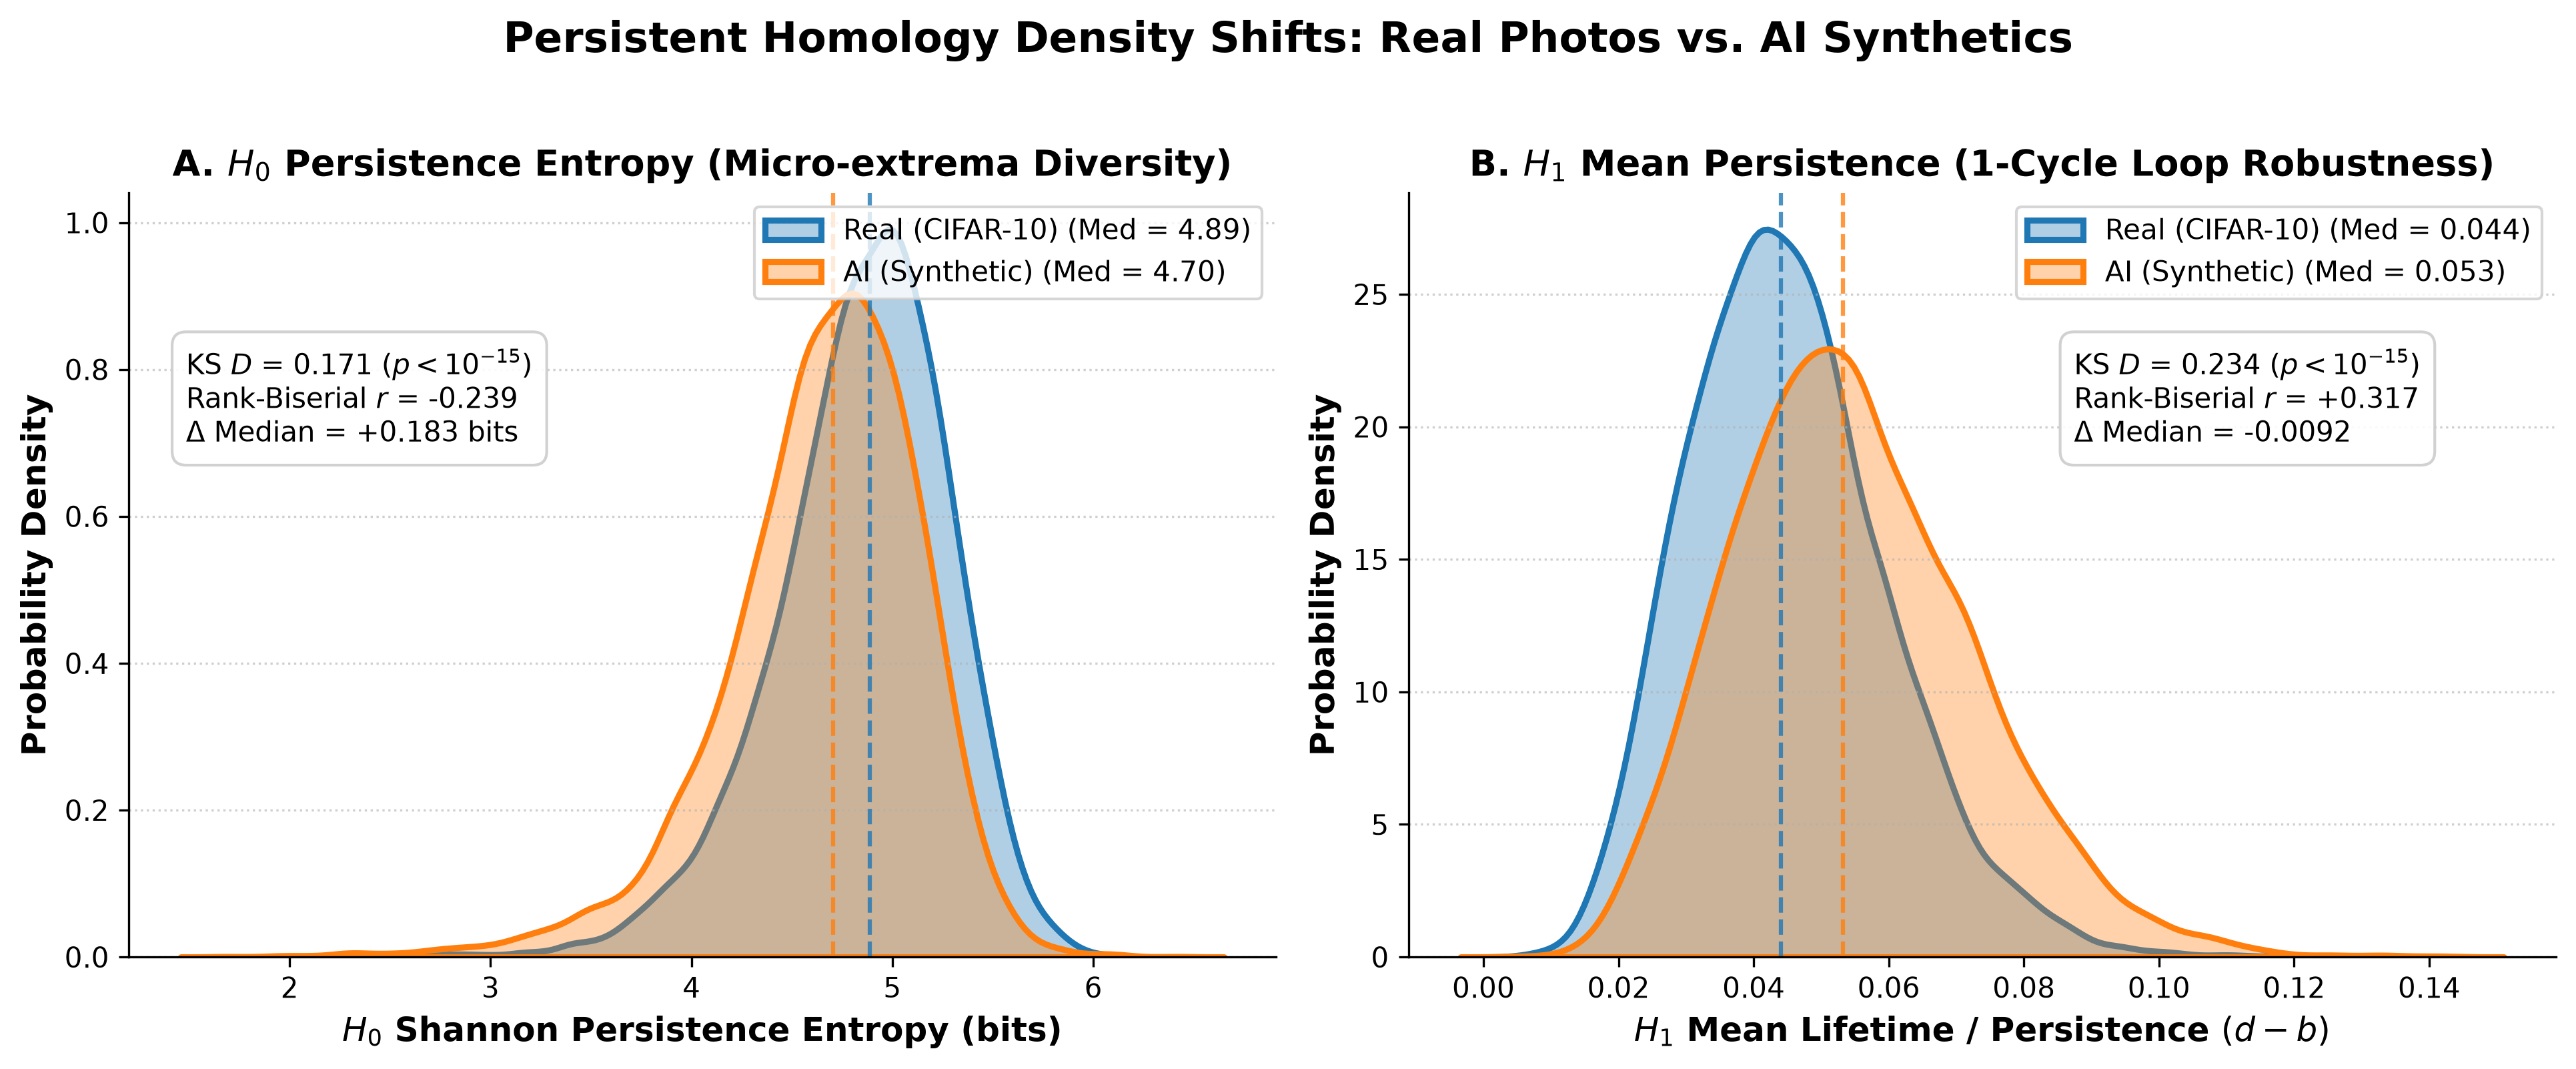
\includegraphics[width=\textwidth]{figures/topological_kde_distributions.png}
    \caption{Kernel Density Estimation of $H_0$ Persistence Entropy and $H_1$ Mean Persistence for Real (blue) vs. AI (orange) images. Dashed lines mark class medians.}
    \label{fig:kde}
\end{figure}

Two critical phenomena emerge from the density distributions:
\begin{enumerate}
    \item \textbf{High-Entropy Real Photography (Panel A)}: Real photographs concentrate systematically towards higher entropy values ($\text{Median} = 4.89$ bits vs. $4.70$ bits for AI; KS $D = 0.171$). Shannon persistence entropy quantifies the uniformity of feature lifetimes: higher entropy reflects a more even normalized lifetime distribution and/or more features, rather than necessarily a broader spectrum of scales.
    \item \textbf{Heavy-Tailed Synthetic $H_1$ Persistence (Panel B)}: While the real photographic distribution peaks sharply at $\mu \approx 0.044$ and decays rapidly, the AI synthetic distribution exhibits an elevated median ($\text{Median} = 0.053$; KS $D = 0.234$; Rank-Biserial $r = +0.317$) with substantial probability mass extending beyond $0.080$.
\end{enumerate}

\subsection{Violin Distributions}
Figure~\ref{fig:violin} illustrates the full quartile structures, medians, and density envelopes.

\begin{figure}[H]
    \centering
    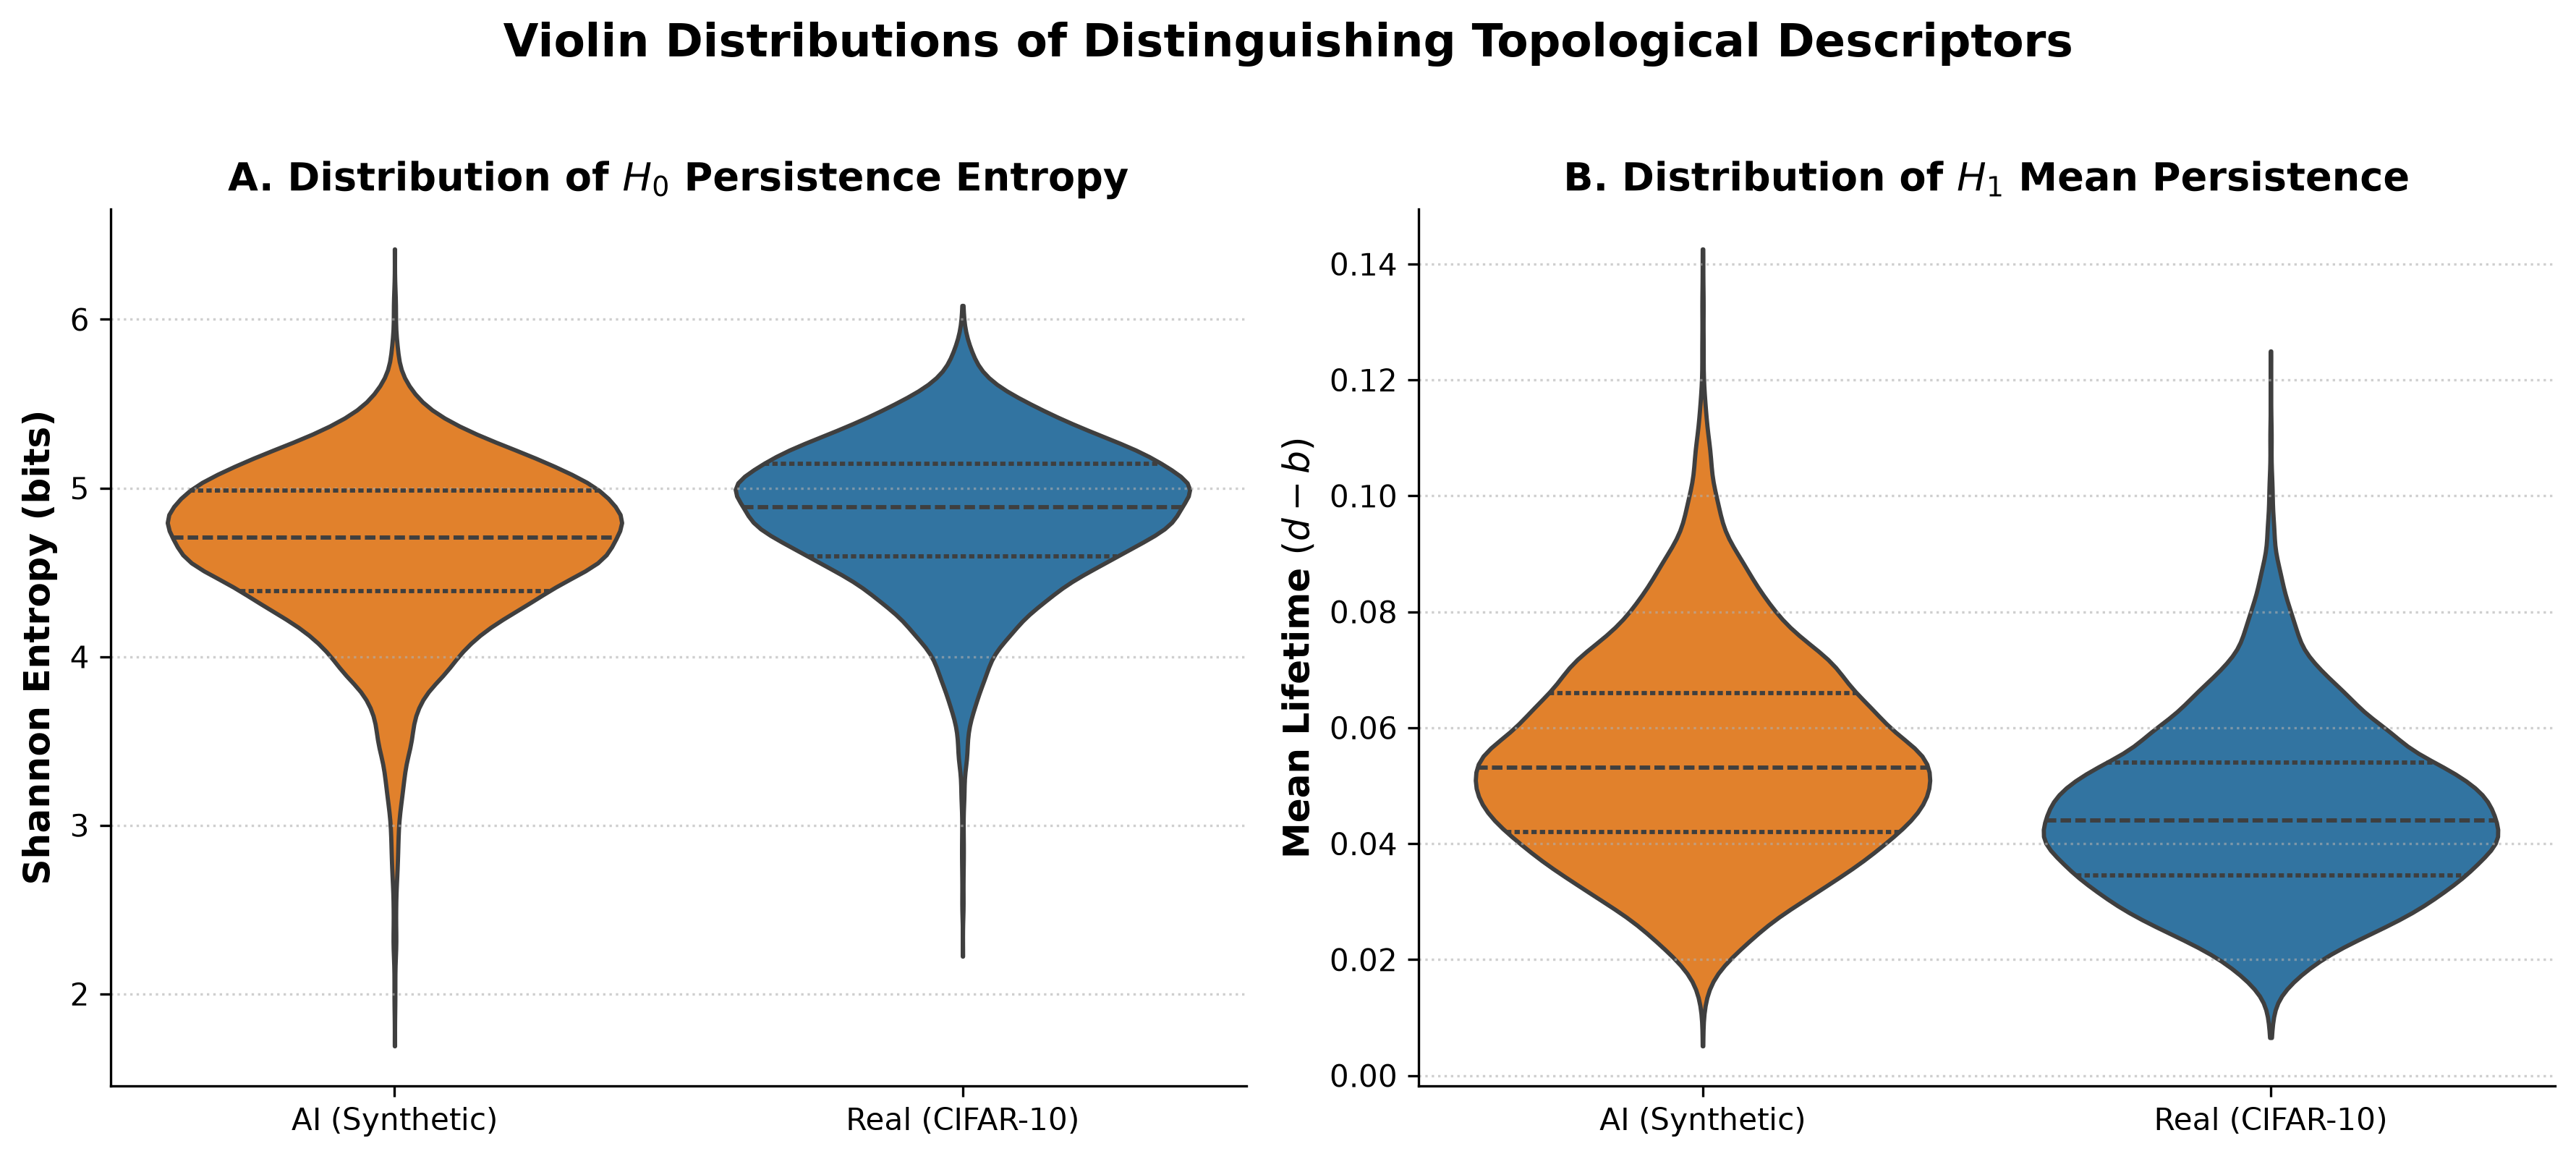
\includegraphics[width=\textwidth]{figures/topological_violin_distributions.png}
    \caption{Violin plots illustrating probability density envelopes and quartile partitions (horizontal dashed lines mark the 25th, 50th, and 75th percentiles).}
    \label{fig:violin}
\end{figure}

The violin geometry highlights an asymmetry in generative artifacts:
\begin{itemize}
    \item In $H_0$ entropy, the AI distribution displays a long, attenuated lower tail reaching down to $\approx 1.8$ bits, indicating concentration of normalized lifetime mass in fewer features for some images; its physical cause is not identified here.
    \item In $H_1$ persistence, the 75th percentile of the AI class ($0.066$) is higher than the real median; the class distributions nevertheless overlap substantially.
\end{itemize}

\subsection{The 2D Topological Phase Space: ``The Shape of a Photograph''}
To examine how these two dimensions interact, Figure~\ref{fig:landscape} maps the 2D joint topological phase space spanned by $H_0$ persistence entropy ($x$-axis) and $H_1$ mean persistence ($y$-axis).

\begin{figure}[H]
    \centering
    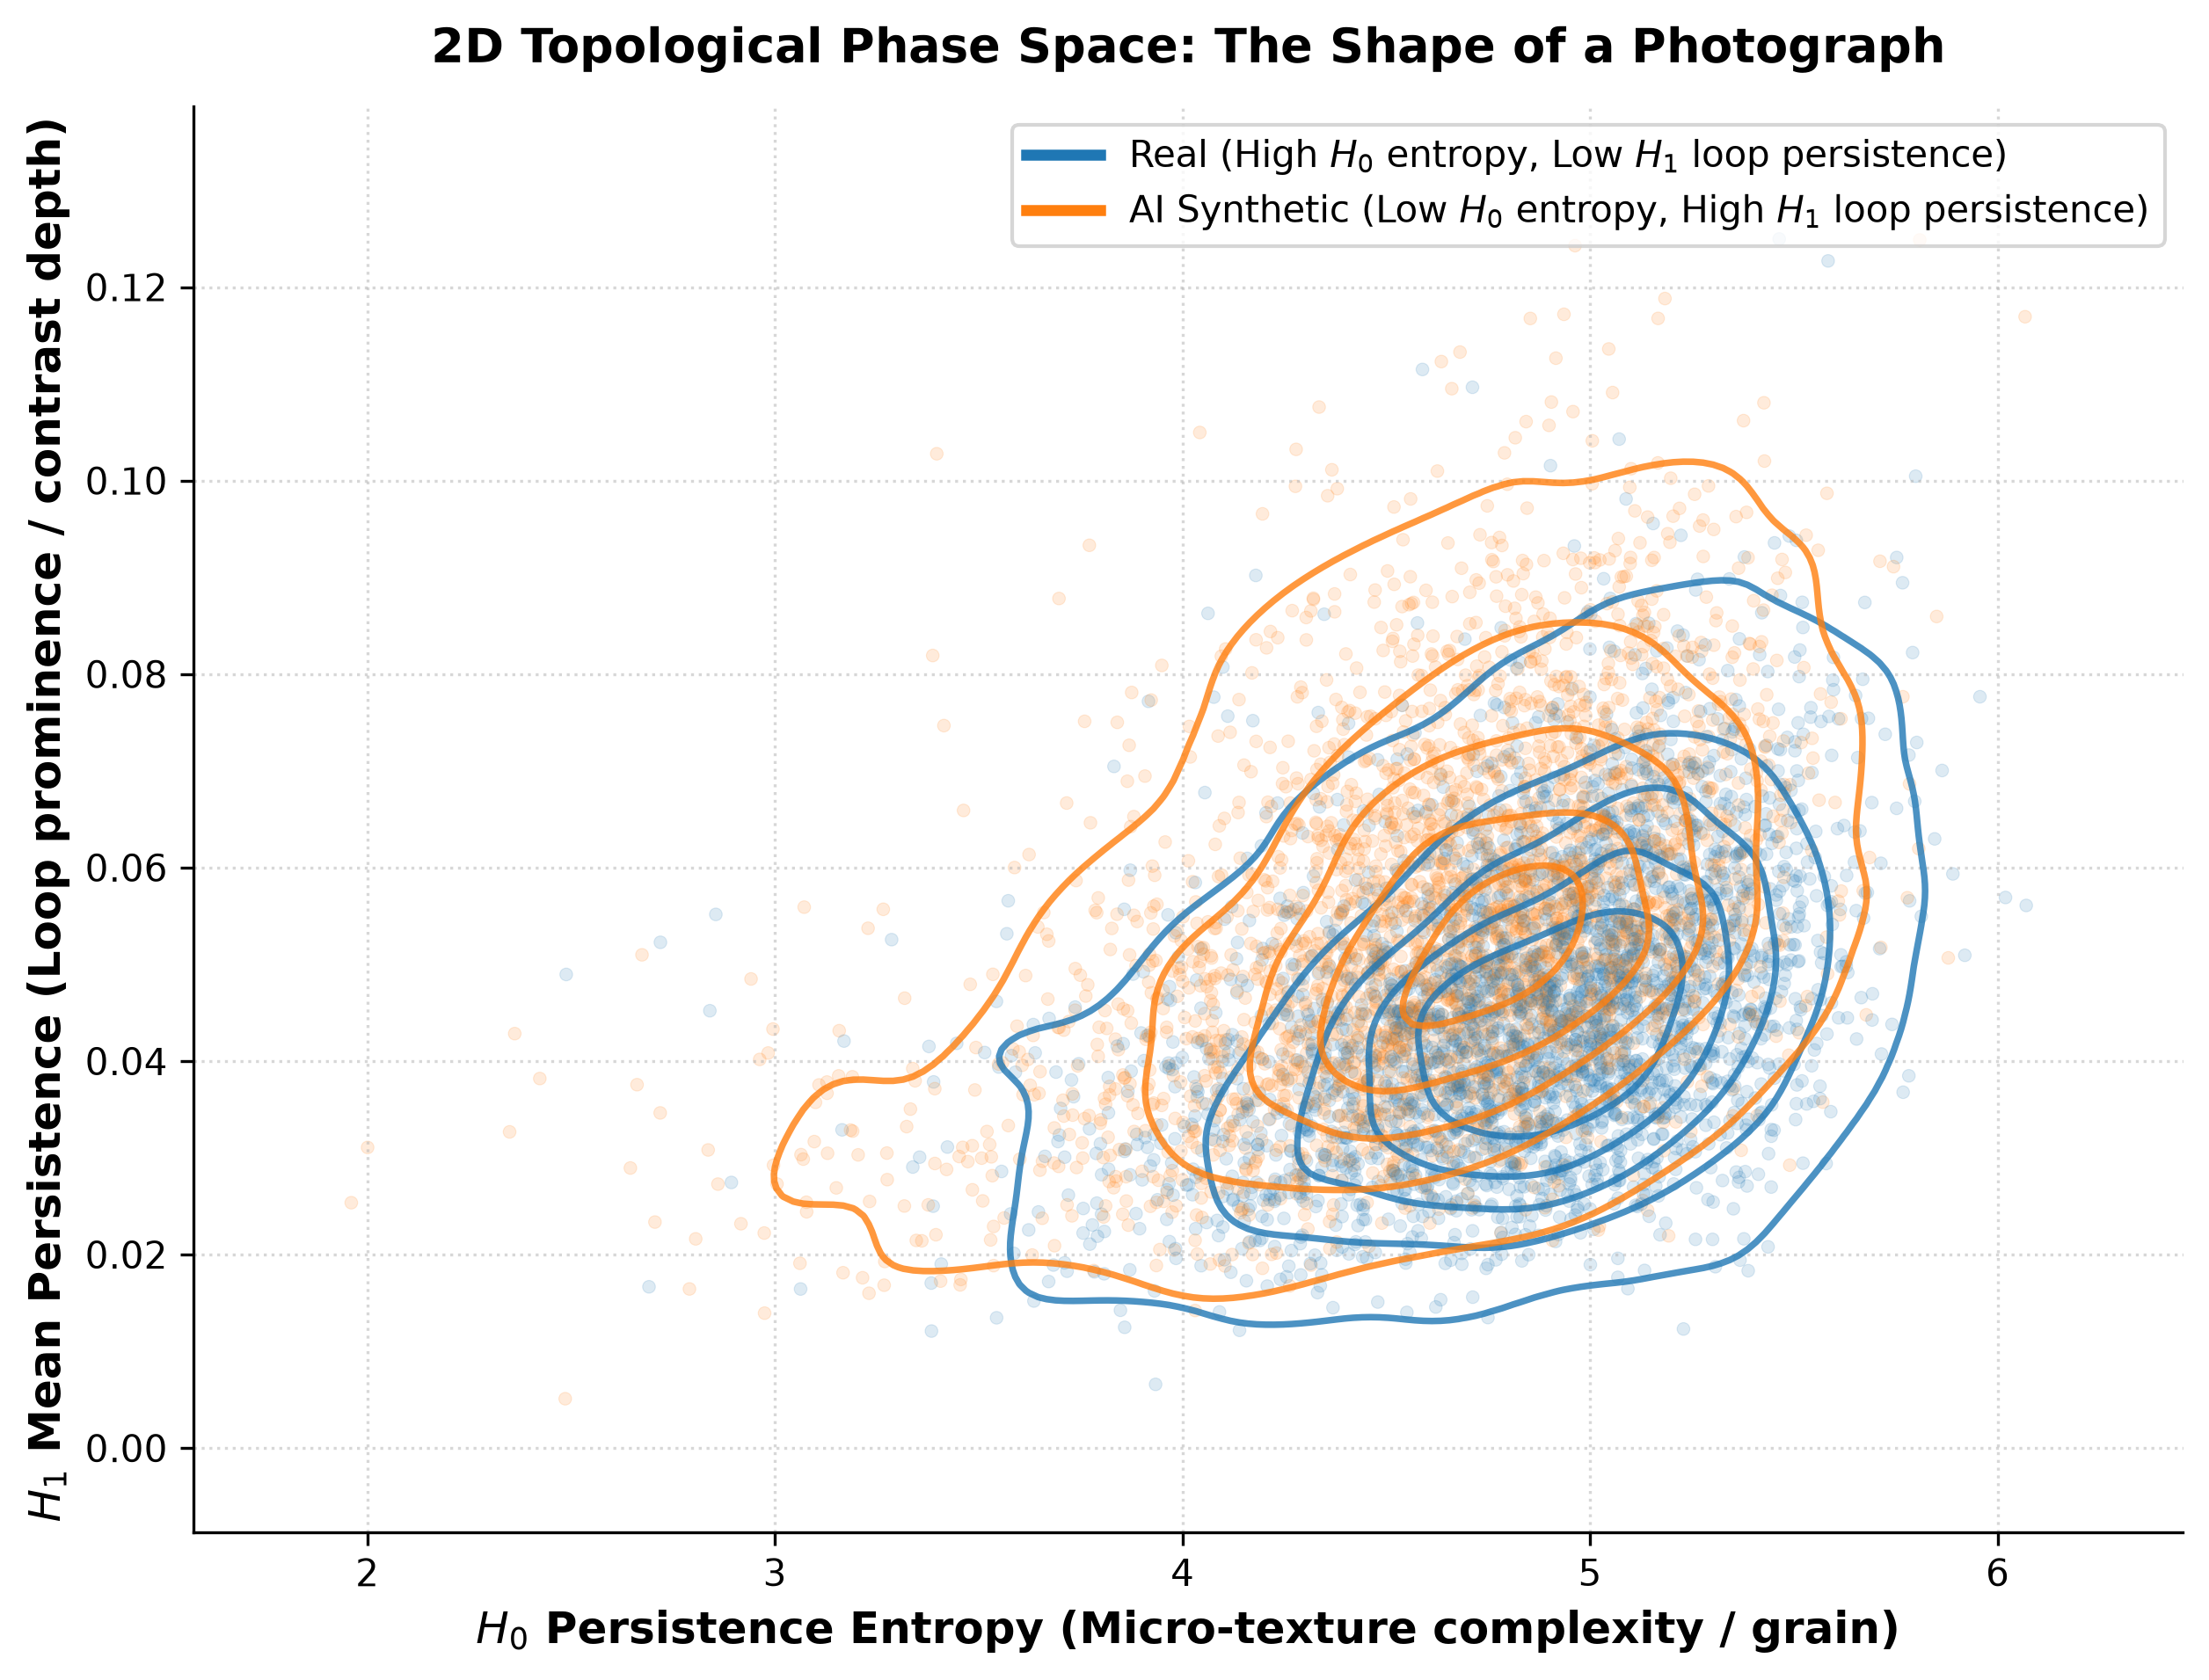
\includegraphics[width=0.85\textwidth]{figures/topological_2d_landscape.png}
    \caption{2D Topological Phase Space ($H_0$ Entropy vs. $H_1$ Mean Persistence) showing bivariate kernel density contours underlaid with individual sample scatters.}
    \label{fig:landscape}
\end{figure}

The phase space reveals distinct clustering behaviors:
\begin{itemize}
    \item \textbf{The Real Photographic Cluster}: Real photographs concentrate tightly in the high-$H_0$-entropy, low-$H_1$-persistence regime (lower-right region). This is an empirical region in the two-feature plot, not an identified physical manifold or a measurement of sensor noise.
    \item \textbf{The Synthetic Diffusion Dispersion}: Synthetic images drift into the upper and upper-left regimes. In this dataset the synthetic sample tends toward lower $H_0$ entropy and higher $H_1$ mean persistence, with substantial overlap with real images.
\end{itemize}

% ==============================================================================
\section{Machine Learning Classification Benchmark}
% ==============================================================================

To rigorously test whether persistent homology features alone provide sufficient discriminative power for automated forensics, we implement a machine learning classification benchmark.

\subsection{Experimental Design and Validation Protocol}
\begin{enumerate}
    \item \textbf{Feature Isolation}: Classifiers are trained \textit{exclusively} on the 16 extracted topological scalar descriptors:
    \begin{equation}
    \begin{split}
        \mathbf{x} = \big[ & N_0, N_1, N_{\text{total}}, L_{\text{total}}(H_0), L_{\text{total}}(H_1), L_{\text{total}}, L_{\max}(H_0), L_{\max}(H_1), \\
        & L_{\max}, E(H_0), E(H_1), E_{\text{total}}, \mu_0, \mu_1, \sigma_0, \sigma_1 \big]^T
    \end{split}
    \end{equation}
    All raw pixel statistics (\texttt{pixel\_mean}, \texttt{pixel\_std}, etc.) are strictly excluded to evaluate the unassisted discriminative capacity of topology.
    \item \textbf{Dataset Partitioning}: The dataset of $N=20{,}000$ images is partitioned into a training set of $16{,}000$ images (80\%, $8{,}000$ real, $8{,}000$ AI) and an internal hold-out test set of $4{,}000$ images (20\%, $2{,}000$ real, $2{,}000$ AI) using stratified sampling.
    \item \textbf{Cross-Validation}: On the training split, 5-fold Stratified Cross-Validation is executed. Continuous models (Logistic Regression and SVM) incorporate standard feature scaling (\texttt{StandardScaler}) fitted strictly within each cross-validation fold to prevent data leakage.
    \item \textbf{Model Architectures}: We evaluate six canonical, lightweight architectures:
    \begin{itemize}[noitemsep]
        \item \textbf{Regularized Logistic Regression (L2)}: Convex linear baseline with $C=1.0$ and L-BFGS solver.
        \item \textbf{Linear Support Vector Machine (Linear SVM)}: Maximum-margin linear hyperplane with Platt-calibrated probabilities~\cite{cortes1995support}.
        \item \textbf{Radial Basis Function Support Vector Machine (RBF SVM)}: Non-linear kernel SVM capturing curved manifold geometry.
        \item \textbf{Random Forest Classifier}: Ensemble of 300 decorrelated decision trees with max depth 12~\cite{breiman2001random}.
        \item \textbf{XGBoost Classifier}: Extreme gradient boosting using histogram-based split optimization (300 estimators, depth 6, $\eta=0.05$, subsampling 0.8)~\cite{chen2016xgboost}.
        \item \textbf{LightGBM Classifier}: Leaf-wise gradient boosted trees with histogram binning (300 estimators, depth 6, $\eta=0.05$)~\cite{ke2017lightgbm}.
    \end{itemize}
\end{enumerate}

\subsection{Benchmark Performance Results}
Table~\ref{tab:ml_benchmark} presents the 5-fold cross-validation performance alongside comprehensive hold-out test metrics ($N_{\text{test}} = 4{,}000$).

\begin{table}[H]
\centering
\small
\caption{Classification benchmark using strictly 16 topological features ($N_{\text{train}} = 16{,}000, N_{\text{test}} = 4{,}000$).}
\label{tab:ml_benchmark}
\resizebox{\textwidth}{!}{%
\begin{tabular}{lcccccccc}
\toprule
\textbf{Model} & \textbf{5-Fold CV Acc.} & \textbf{5-Fold CV AUC} & \textbf{Test Acc.} & \textbf{Test AUC} & \textbf{Test F1} & \textbf{Precision} & \textbf{Recall} & \textbf{Brier Score} \\
\midrule
Logistic Regression (L2) & $69.99\% \pm 0.52\%$ & $0.7698 \pm 0.0053$ & $68.90\%$ & $0.7646$ & $0.7018$ & $0.6740$ & $0.7320$ & $0.1969$ \\
Linear SVM & $69.92\% \pm 0.47\%$ & $0.7697 \pm 0.0052$ & $68.90\%$ & $0.7644$ & $0.7015$ & $0.6744$ & $0.7310$ & $0.1970$ \\
RBF SVM & $\mathbf{70.72\% \pm 0.32\%}$ & $\mathbf{0.7811 \pm 0.0047}$ & $\mathbf{70.03\%}$ & $0.7755$ & $\mathbf{0.7138}$ & $\mathbf{0.6830}$ & $0.7475$ & $0.1932$ \\
Random Forest & $70.56\% \pm 0.78\%$ & $0.7758 \pm 0.0051$ & $69.55\%$ & $0.7750$ & $0.7078$ & $0.6804$ & $0.7375$ & $0.1923$ \\
XGBoost & $70.41\% \pm 0.49\%$ & $0.7765 \pm 0.0053$ & $69.73\%$ & $0.7756$ & $0.7074$ & $0.6844$ & $0.7320$ & $0.1924$ \\
LightGBM & $70.36\% \pm 0.30\%$ & $0.7775 \pm 0.0051$ & $69.95\%$ & $\mathbf{0.7789}$ & $0.7135$ & $0.6817$ & $\mathbf{0.7485}$ & $\mathbf{0.1911}$ \\
\bottomrule
\end{tabular}%
}
\end{table}

\begin{figure}[H]
    \centering
    \begin{subfigure}[b]{0.48\textwidth}
        \centering
        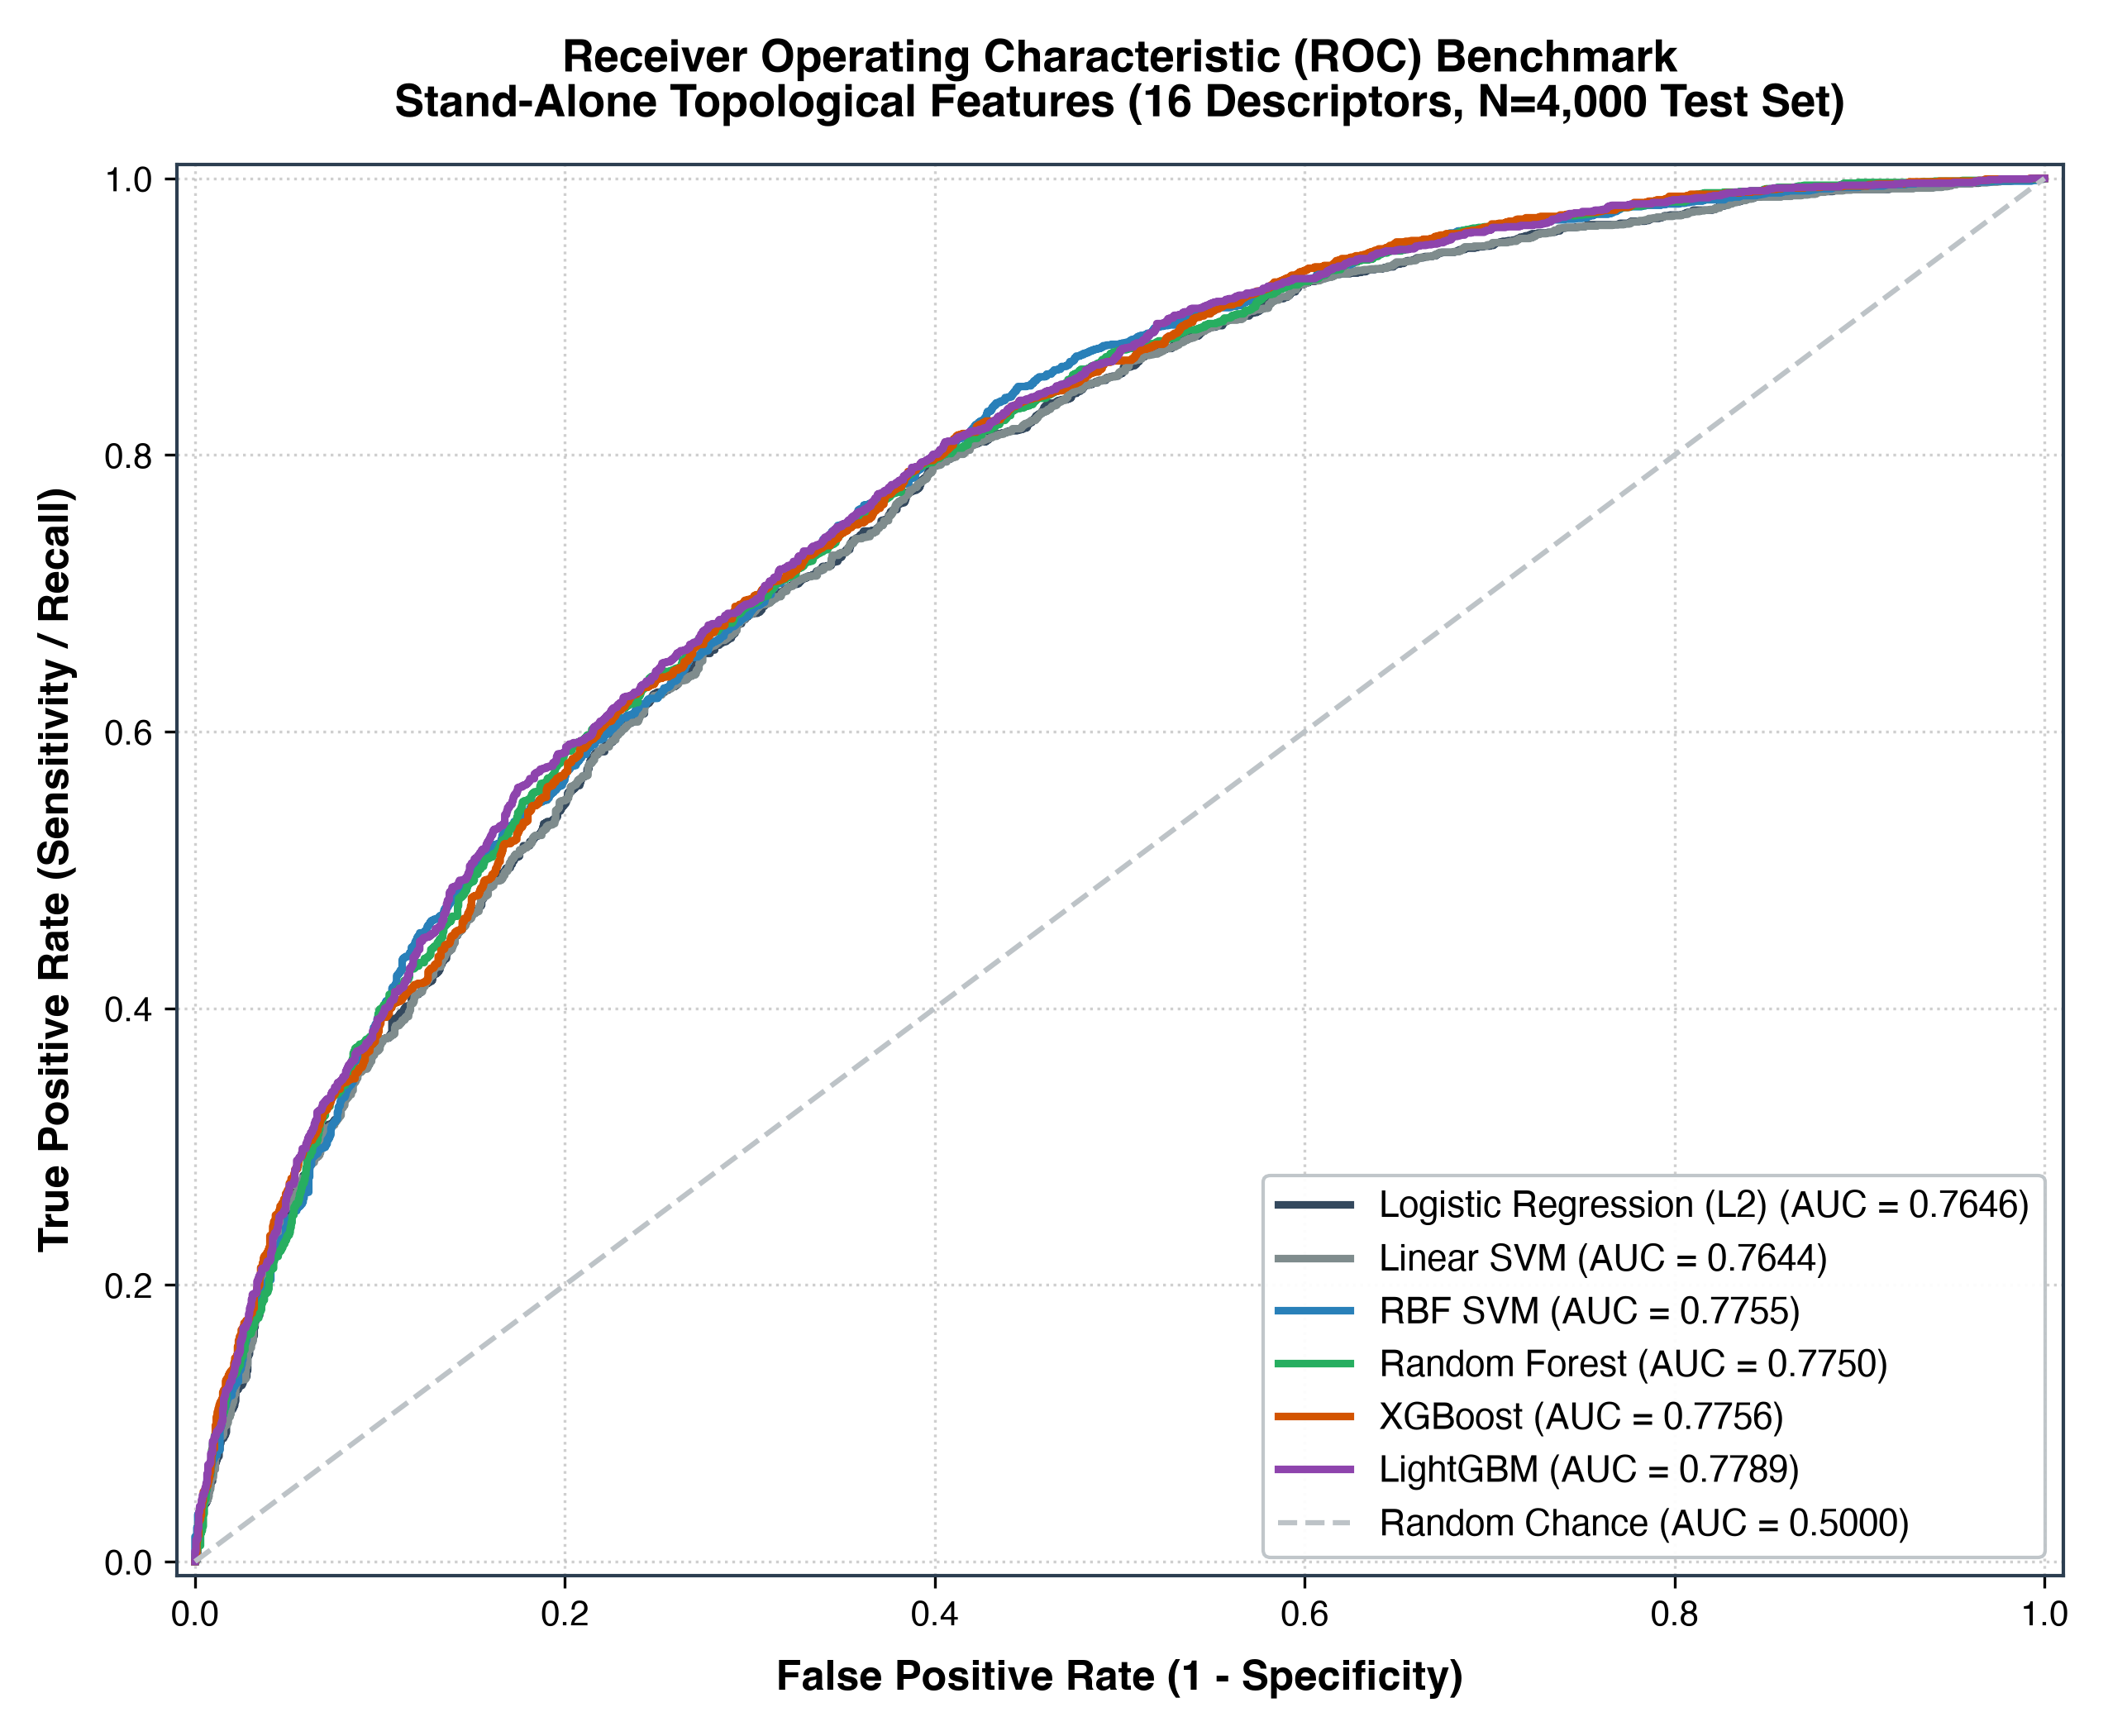
\includegraphics[width=\textwidth]{figures/roc_curves_comparison.png}
        \caption{Receiver Operating Characteristic (ROC) curves.}
        \label{fig:roc_curves}
    \end{subfigure}
    \hfill
    \begin{subfigure}[b]{0.48\textwidth}
        \centering
        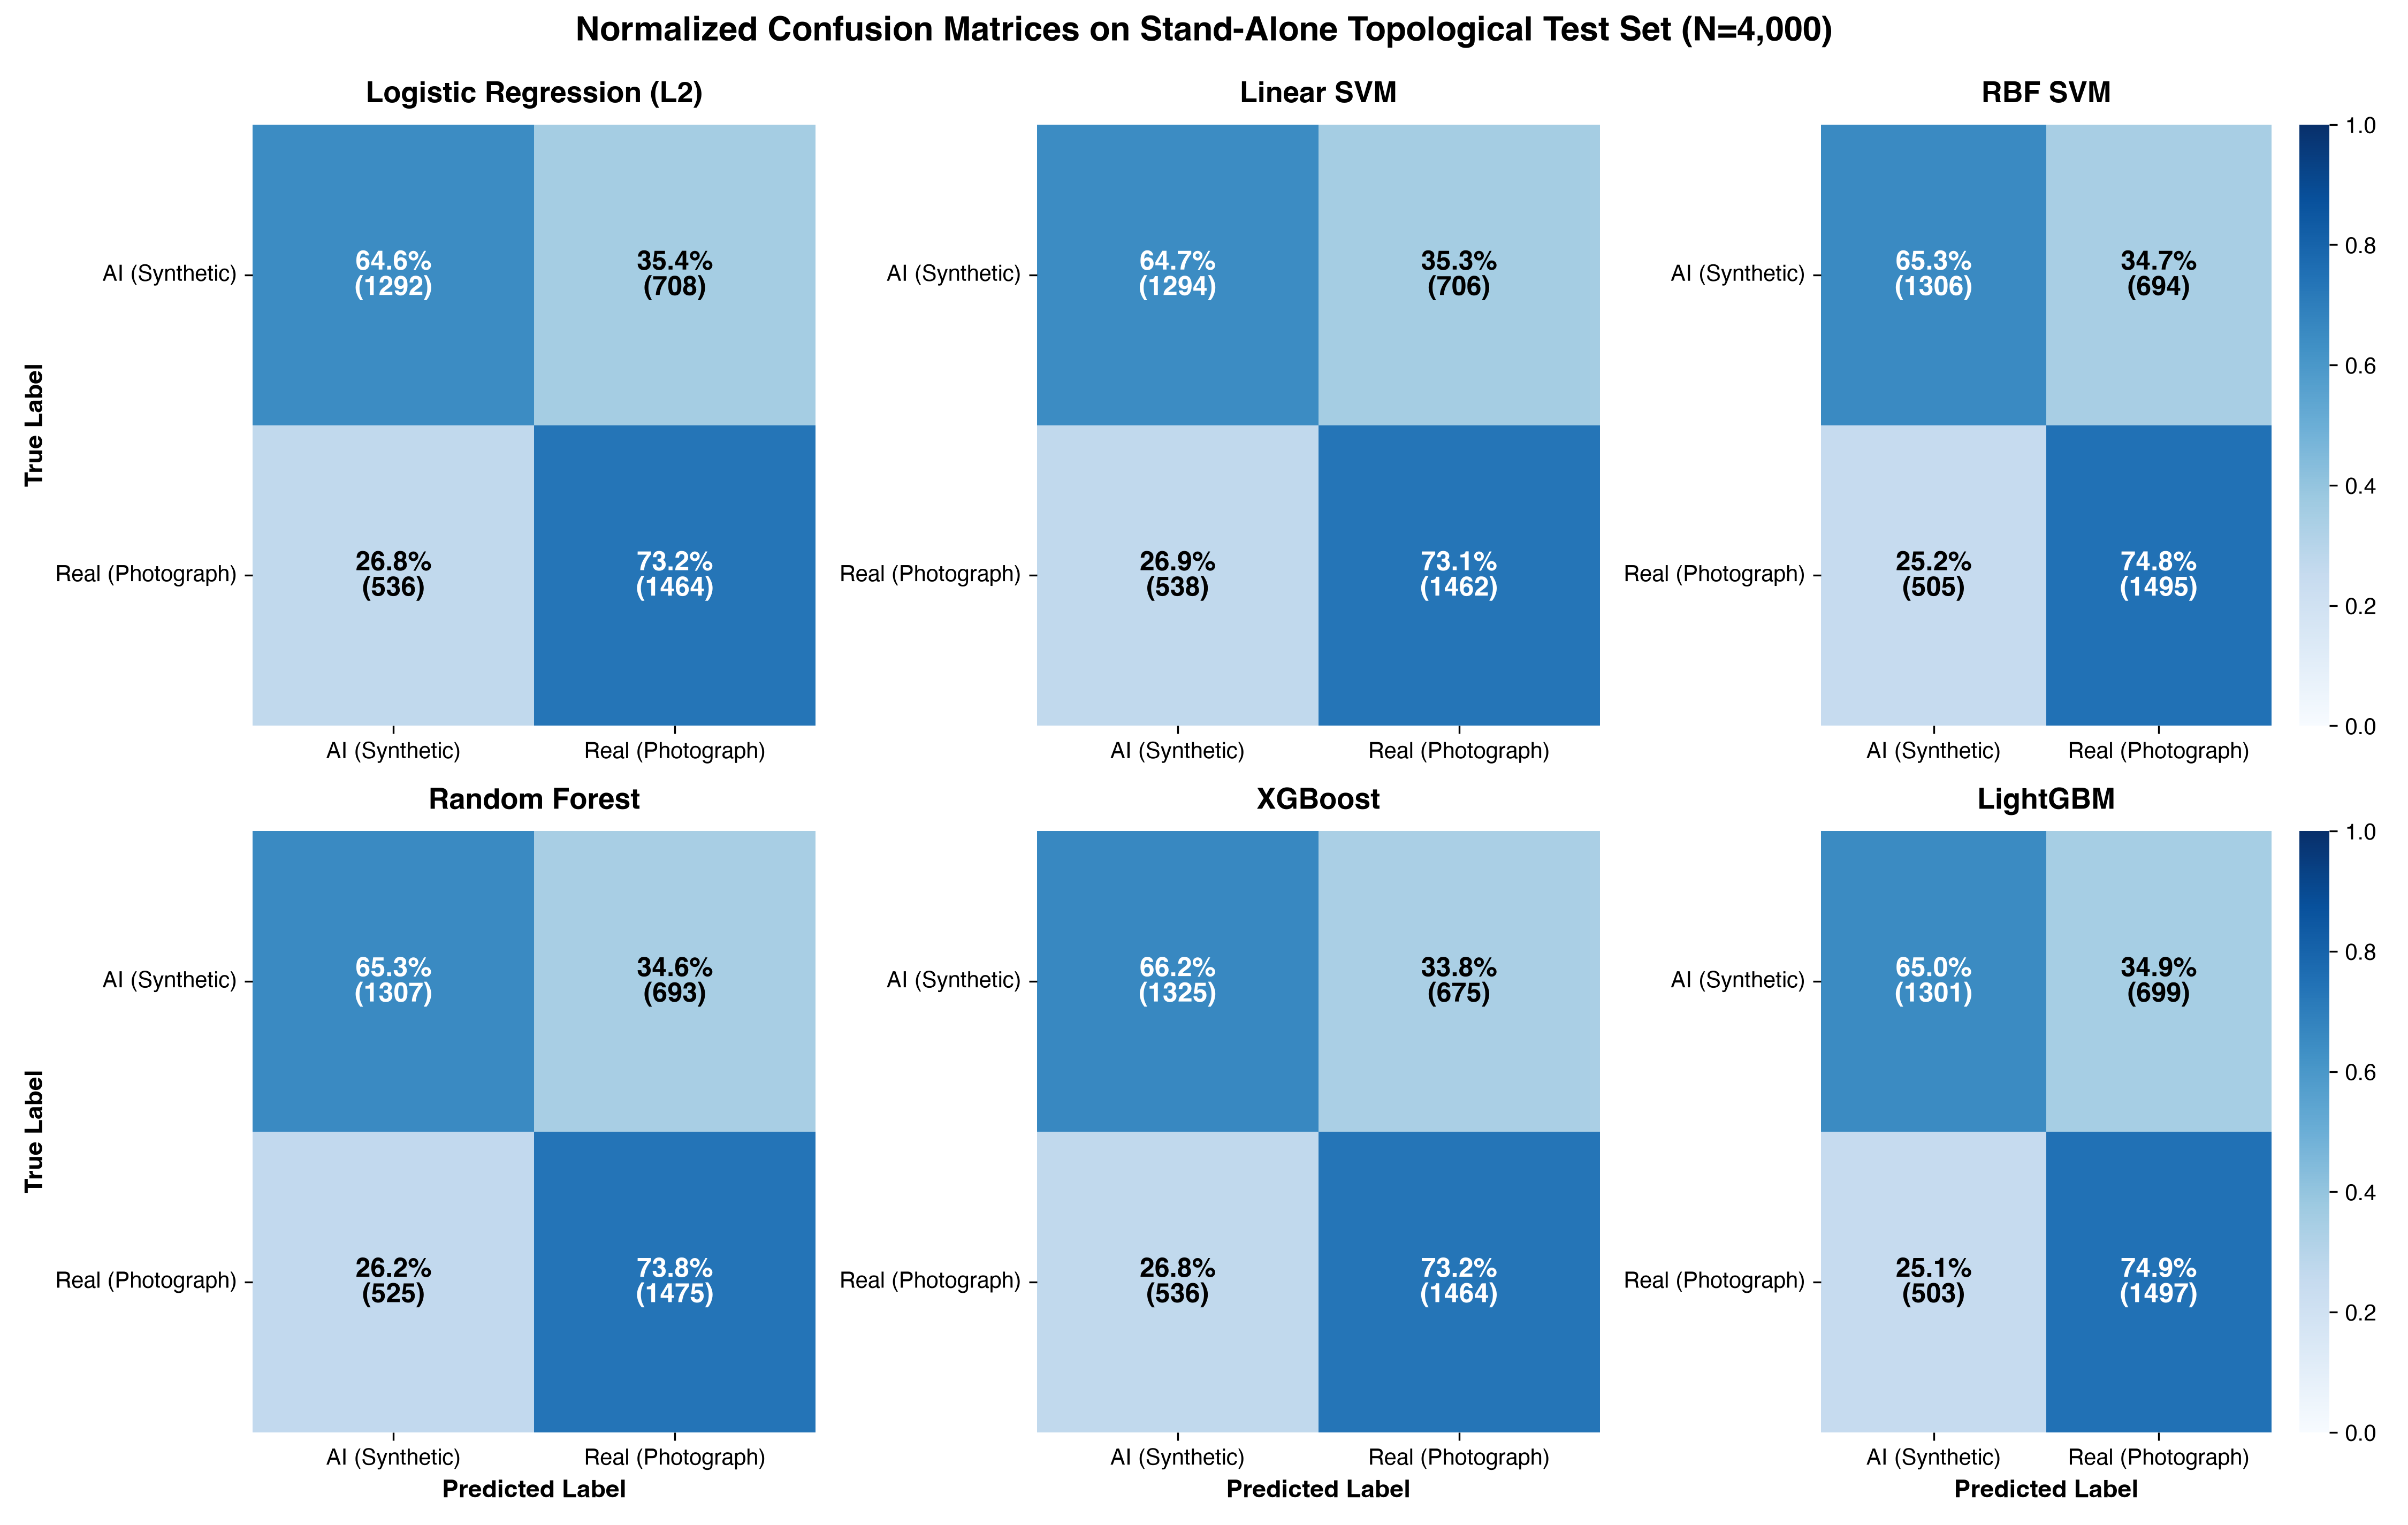
\includegraphics[width=\textwidth]{figures/confusion_matrices.png}
        \caption{Normalized test confusion matrices.}
        \label{fig:confusion_matrices}
    \end{subfigure}
    \caption{Classification benchmark evaluation on hold-out test split ($N=4{,}000$): (a) overlaid ROC curves showing near-identical discrimination across architectures, and (b) normalized confusion matrices illustrating balanced class sensitivities.}
    \label{fig:ml_eval}
\end{figure}

\subsection{Analysis of Stand-Alone Discriminative Efficacy}
Three foundational insights arise from the benchmark:
\begin{enumerate}
    \item \textbf{Stand-Alone Discriminative Power}: Every single classifier achieves $\sim 70\%$ test accuracy and an ROC-AUC of $0.765$ to $0.779$ using \textit{only 16 topological numbers}. Given that random guessing is $50\%$, and that CIFAKE images are highly compressed ($32 \times 32$), this provides evidence of useful topological features on this split. The features are derived from pixel intensities, but the tabular classifiers receive only their summaries. Robustness was not tested.
    \item \textbf{Linear vs. Non-Linear Separability}: While linear models (Logistic Regression and Linear SVM) establish a solid baseline ($68.90\%$ test accuracy, $0.7646$ AUC), non-linear classifiers (RBF SVM, LightGBM, and XGBoost) systematically improve accuracy to $70.03\%$ and AUC to $0.7789$. The observed differences motivate non-linear modeling but do not establish a geometric property of a population decision boundary.
    \item \textbf{Balanced Sensitivity and Specificity}: As evidenced by the confusion matrices (Figure~\ref{fig:confusion_matrices}), models maintain balanced detection rates: for LightGBM, True Positive Rate (Real recall) is $74.9\%$ ($1{,}497 / 2{,}000$) while True Negative Rate (AI specificity) is $65.0\%$ ($1{,}301 / 2{,}000$), showing different sensitivities for the two classes on this split.
\end{enumerate}

% ==============================================================================
\section{Explainability and Topological Attributions via SHAP}
% ==============================================================================

To understand the decision rules formed by non-linear tree ensembles, we employ \textbf{SHAP (SHapley Additive exPlanations)}~\cite{lundberg2017unified}. Based on cooperative game theory, SHAP computes unique additive feature attributions $\Phi_i(x)$ satisfying efficiency, symmetry, dummy, and additivity axioms:
\begin{equation}
    f(x) = \phi_0 + \sum_{i=1}^M \Phi_i(x)
\end{equation}
where $\phi_0 = \mathbb{E}[f(X)]$ is the base value (expected model log-odds output), and $\Phi_i(x)$ is the contribution of feature $i$ towards the prediction for instance $x$. Positive SHAP values push the model toward predicting a \textbf{Real Photograph} ($\hat{y} = 1$), whereas negative SHAP values push toward predicting \textbf{AI Synthetic} ($\hat{y} = 0$).

\subsection{Global Topological Feature Importance}
Figure~\ref{fig:shap_bar} quantifies global feature importance via the mean absolute SHAP value:
\begin{equation}
    I_i = \frac{1}{N_{\text{test}}} \sum_{j=1}^{N_{\text{test}}} |\Phi_i(x_j)|
\end{equation}

\begin{figure}[H]
    \centering
    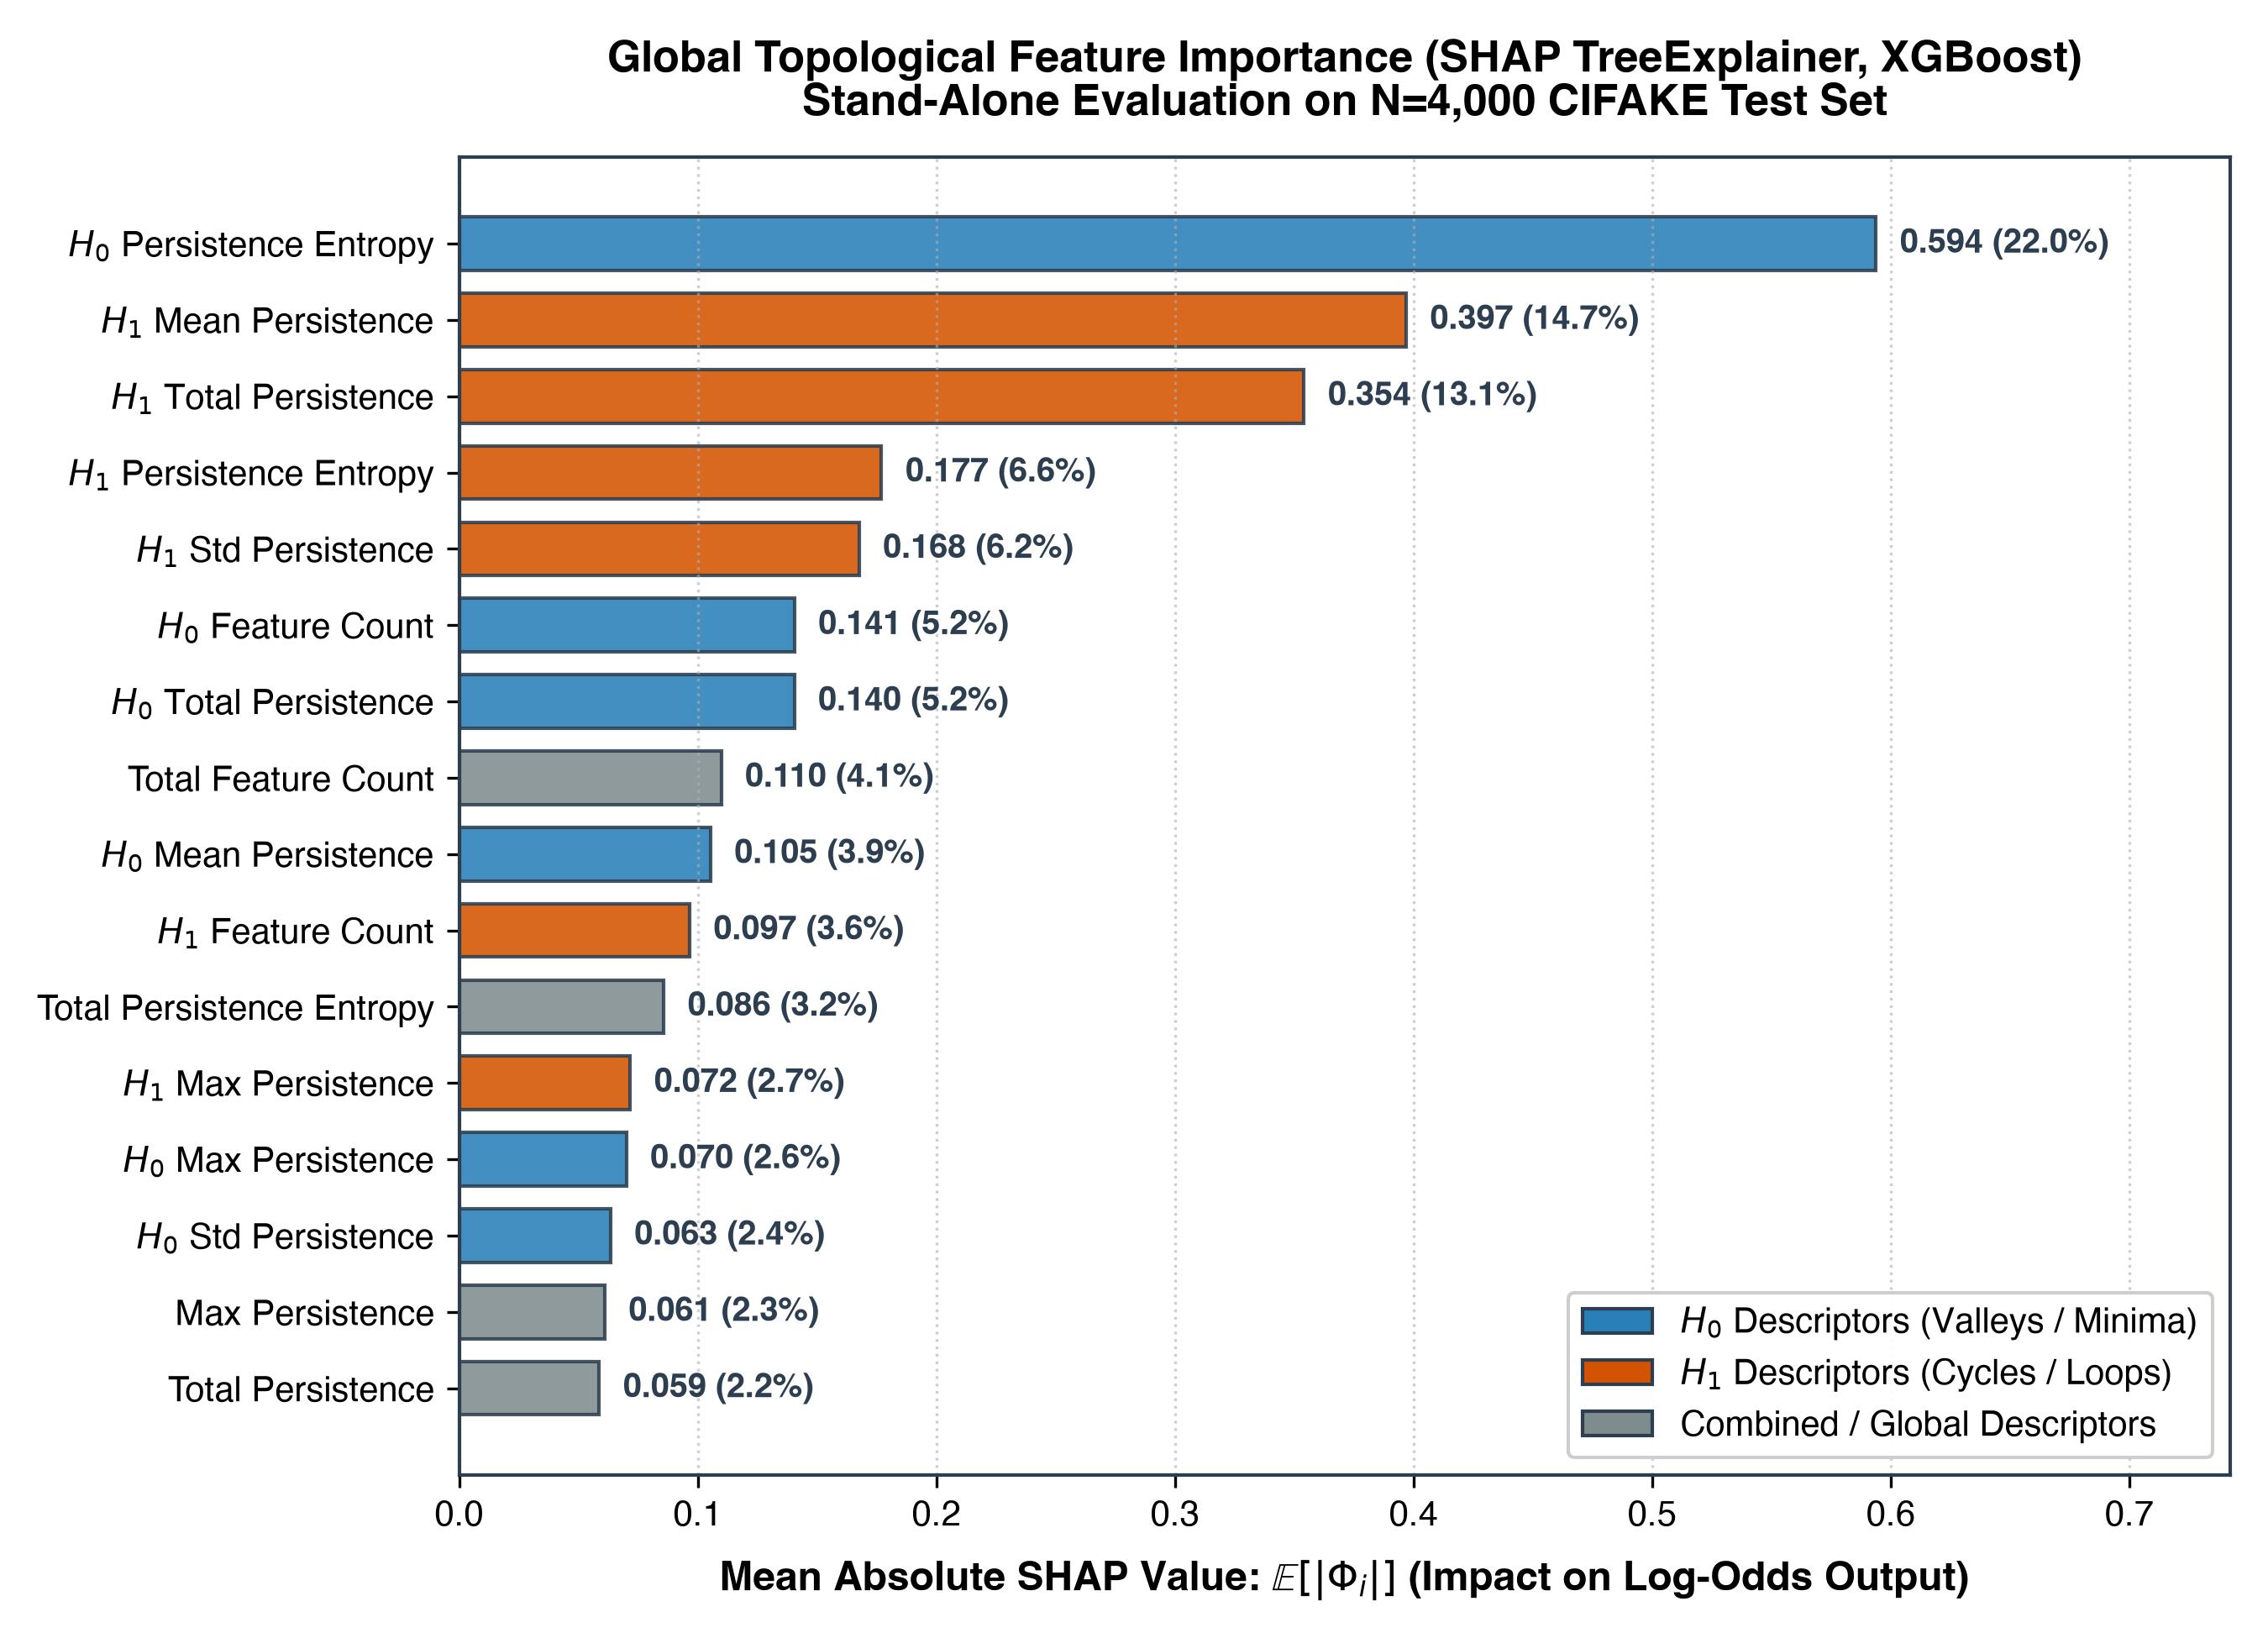
\includegraphics[width=0.88\textwidth]{figures/shap_feature_importance_bar.png}
    \caption{Global topological feature importance ranked by mean absolute SHAP value $\mathbb{E}[|\Phi_i|]$ on the test set ($N=4{,}000$). Colors indicate $H_0$ descriptors (blue), $H_1$ descriptors (orange), and global descriptors (gray).}
    \label{fig:shap_bar}
\end{figure}

The empirical attribution distribution confirms that the topological feature space is strongly hierarchical:
\begin{itemize}
    \item \textbf{$H_0$ Persistence Entropy} is the single most influential feature ($I = 0.5938$), accounting for \textbf{22.05\%} of total decision attribution mass.
    \item \textbf{$H_1$ Mean Persistence} ($I = 0.3969$, \textbf{14.74\%}) and \textbf{$H_1$ Total Persistence} ($I = 0.3541$, \textbf{13.15\%}) represent the second and third most important descriptors.
    \item Together, these top three descriptors constitute \textbf{49.94\%} of the mean-absolute-SHAP attribution total.
\end{itemize}

\subsection{Directional Impact via Beeswarm Summary}
Figure~\ref{fig:shap_beeswarm} depicts the SHAP summary beeswarm plot across the hold-out test set, illustrating how feature magnitudes correlate with decision log-odds.

\begin{figure}[H]
    \centering
    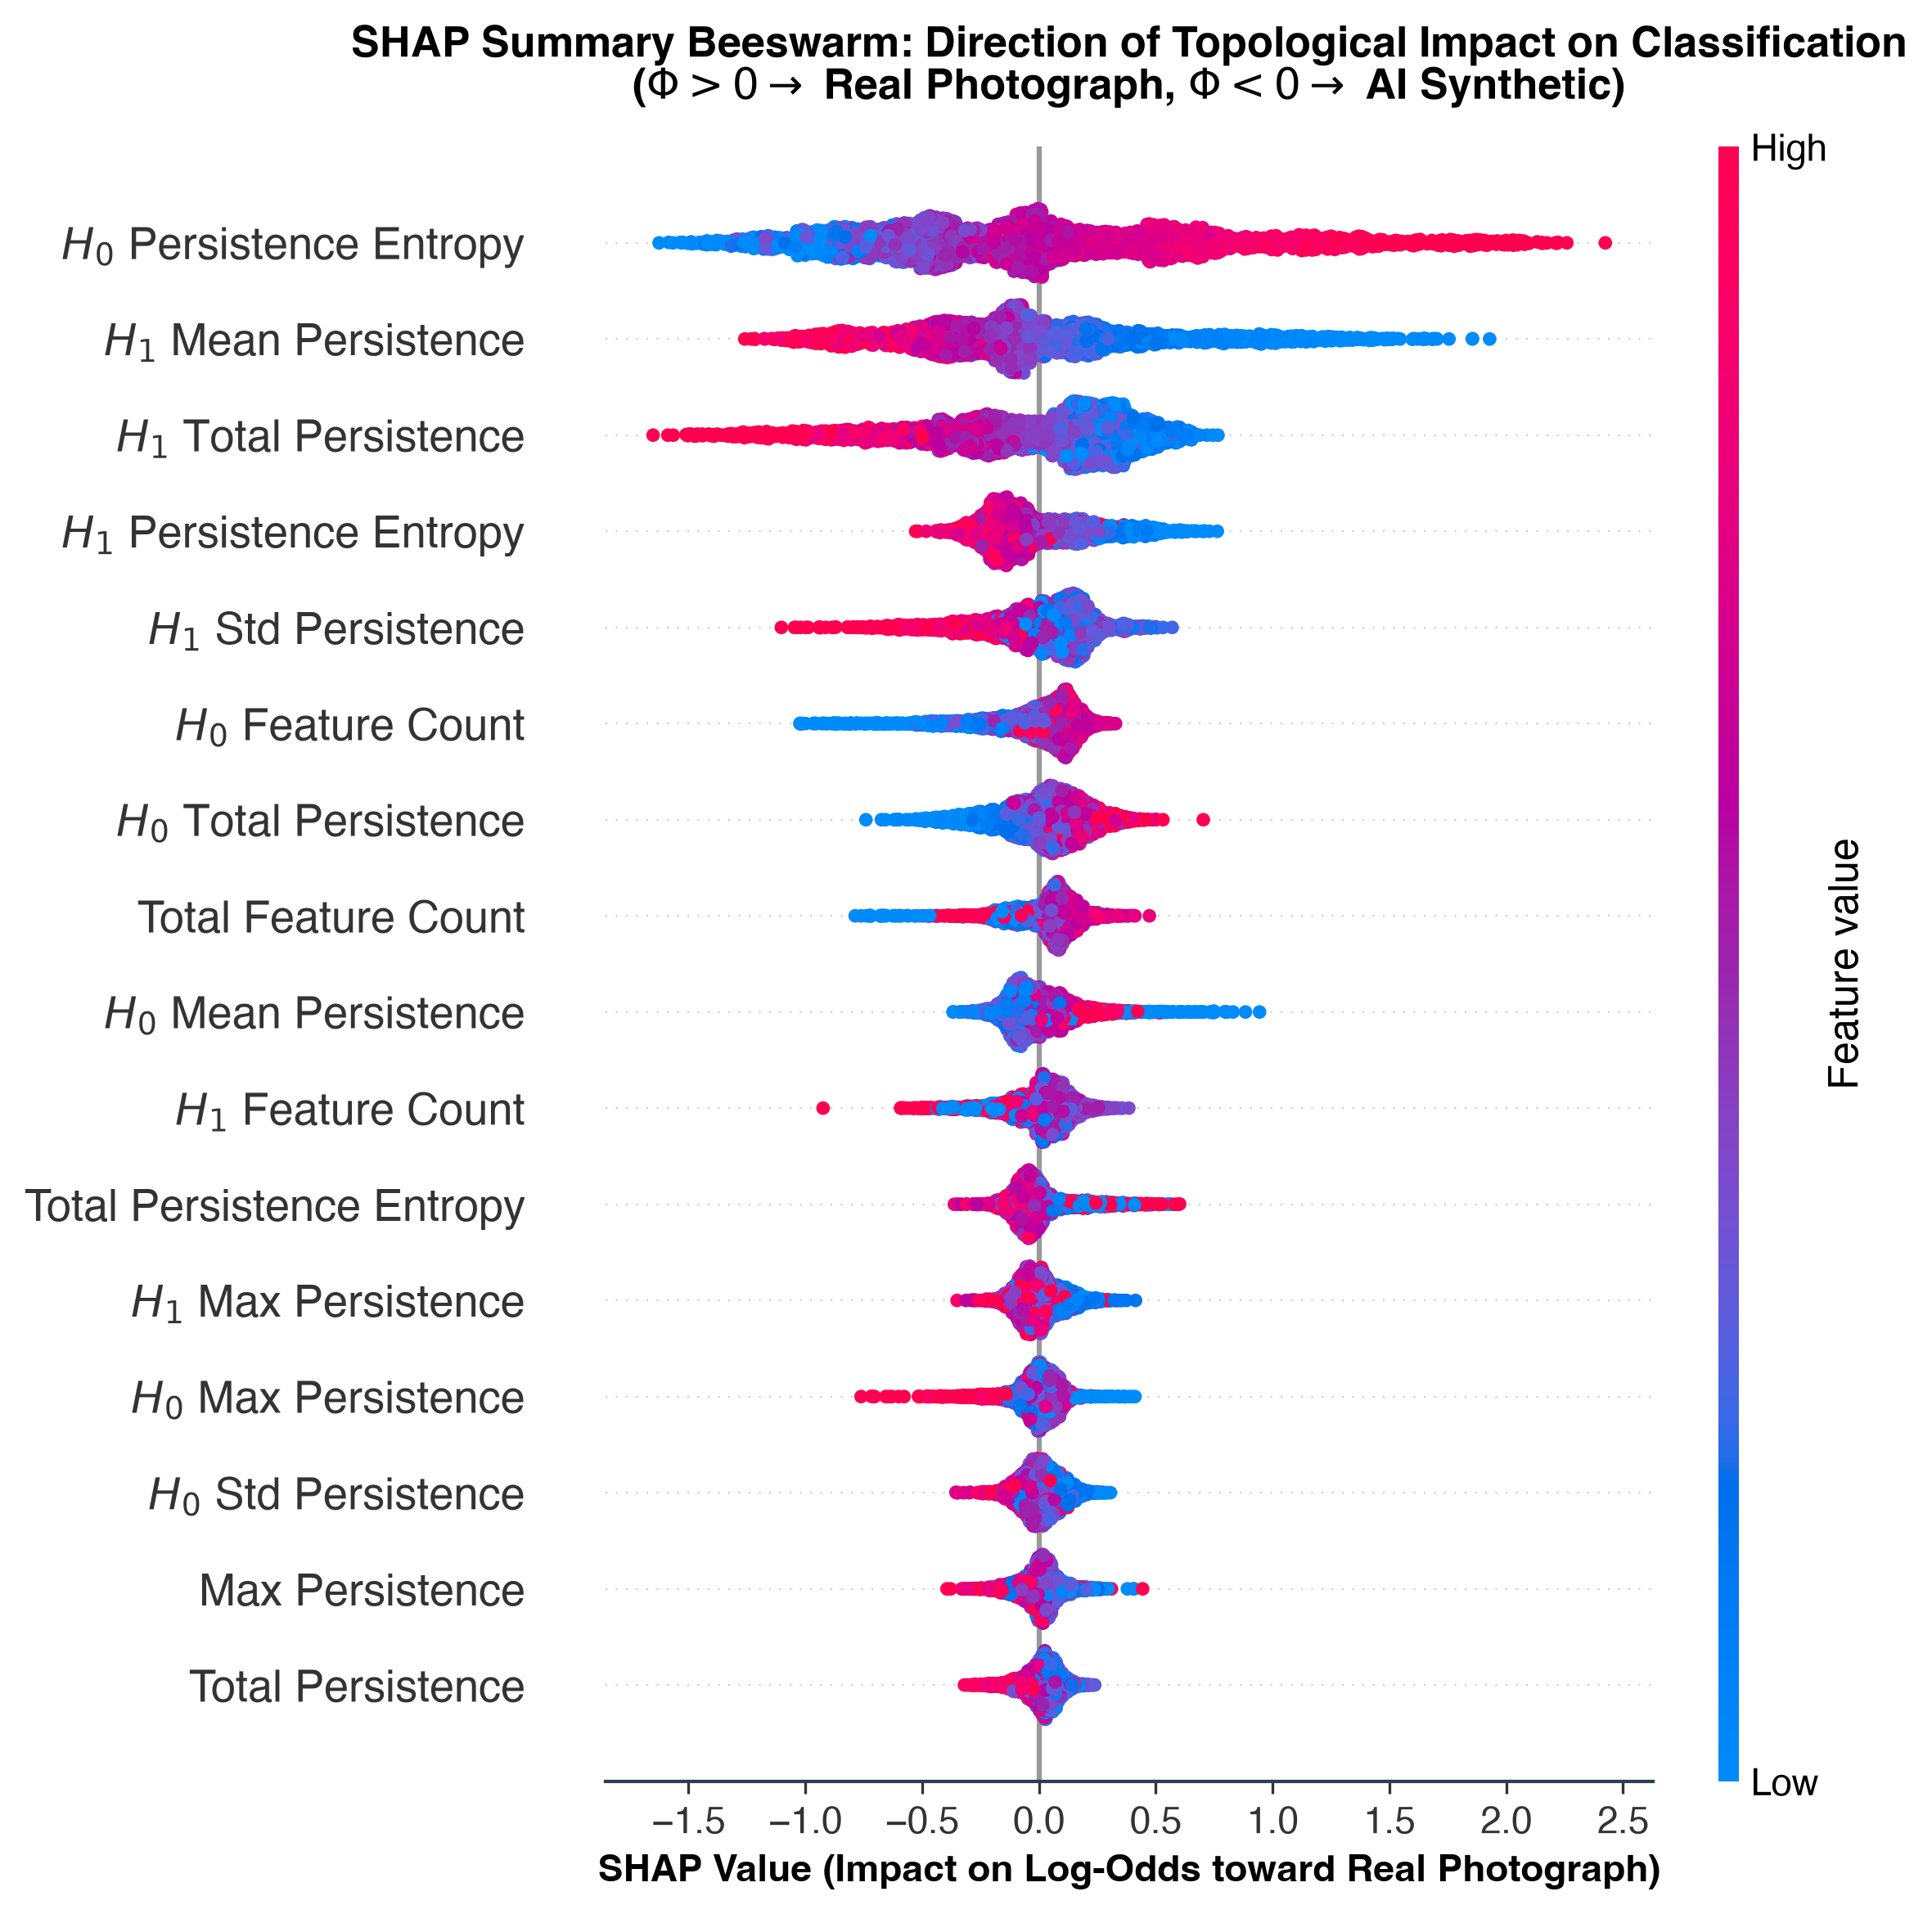
\includegraphics[width=0.90\textwidth]{figures/shap_summary_beeswarm.png}
    \caption{SHAP summary beeswarm plot ($N=4{,}000$). Each point represents one test image; position along the horizontal axis indicates log-odds impact; color indicates feature value (red = high, blue = low).}
    \label{fig:shap_beeswarm}
\end{figure}

The beeswarm plot demonstrates unambiguous directional trends:
\begin{itemize}
    \item \textbf{$H_0$ Persistence Entropy}: High values (red points) tend to have positive SHAP values ($\Phi > 0$), pushing the fitted model toward the real class. Low values (blue points) produce negative attributions pushing predictions to synthetic media.
    \item \textbf{$H_1$ Mean and Total Persistence}: High values (red points) tend toward negative SHAP values ($\Phi < 0$), pushing the fitted model toward the AI class. Low values (blue points) correspond to natural photographic signatures.
\end{itemize}

\subsection{Cross-Feature Interaction Analysis}
TreeSHAP extends to pairwise interaction values $\Phi_{i, j}(x)$ based on the Shapley interaction index:
\begin{equation}
    \Phi_{i, j}(x) = \sum_{S \subseteq N \setminus \{i, j\}} \frac{|S|!(|N| - |S| - 2)!}{2(|N| - 1)!} \left[ f(S \cup \{i, j\}) - f(S \cup \{i\}) - f(S \cup \{j\}) + f(S) \right]
\end{equation}
where $\Phi_{i, i}(x)$ represents the pure main effect, and $\Phi_{i, j}(x)$ ($i \ne j$) quantifies the non-linear interaction effect between feature $i$ and feature $j$.

\begin{figure}[H]
    \centering
    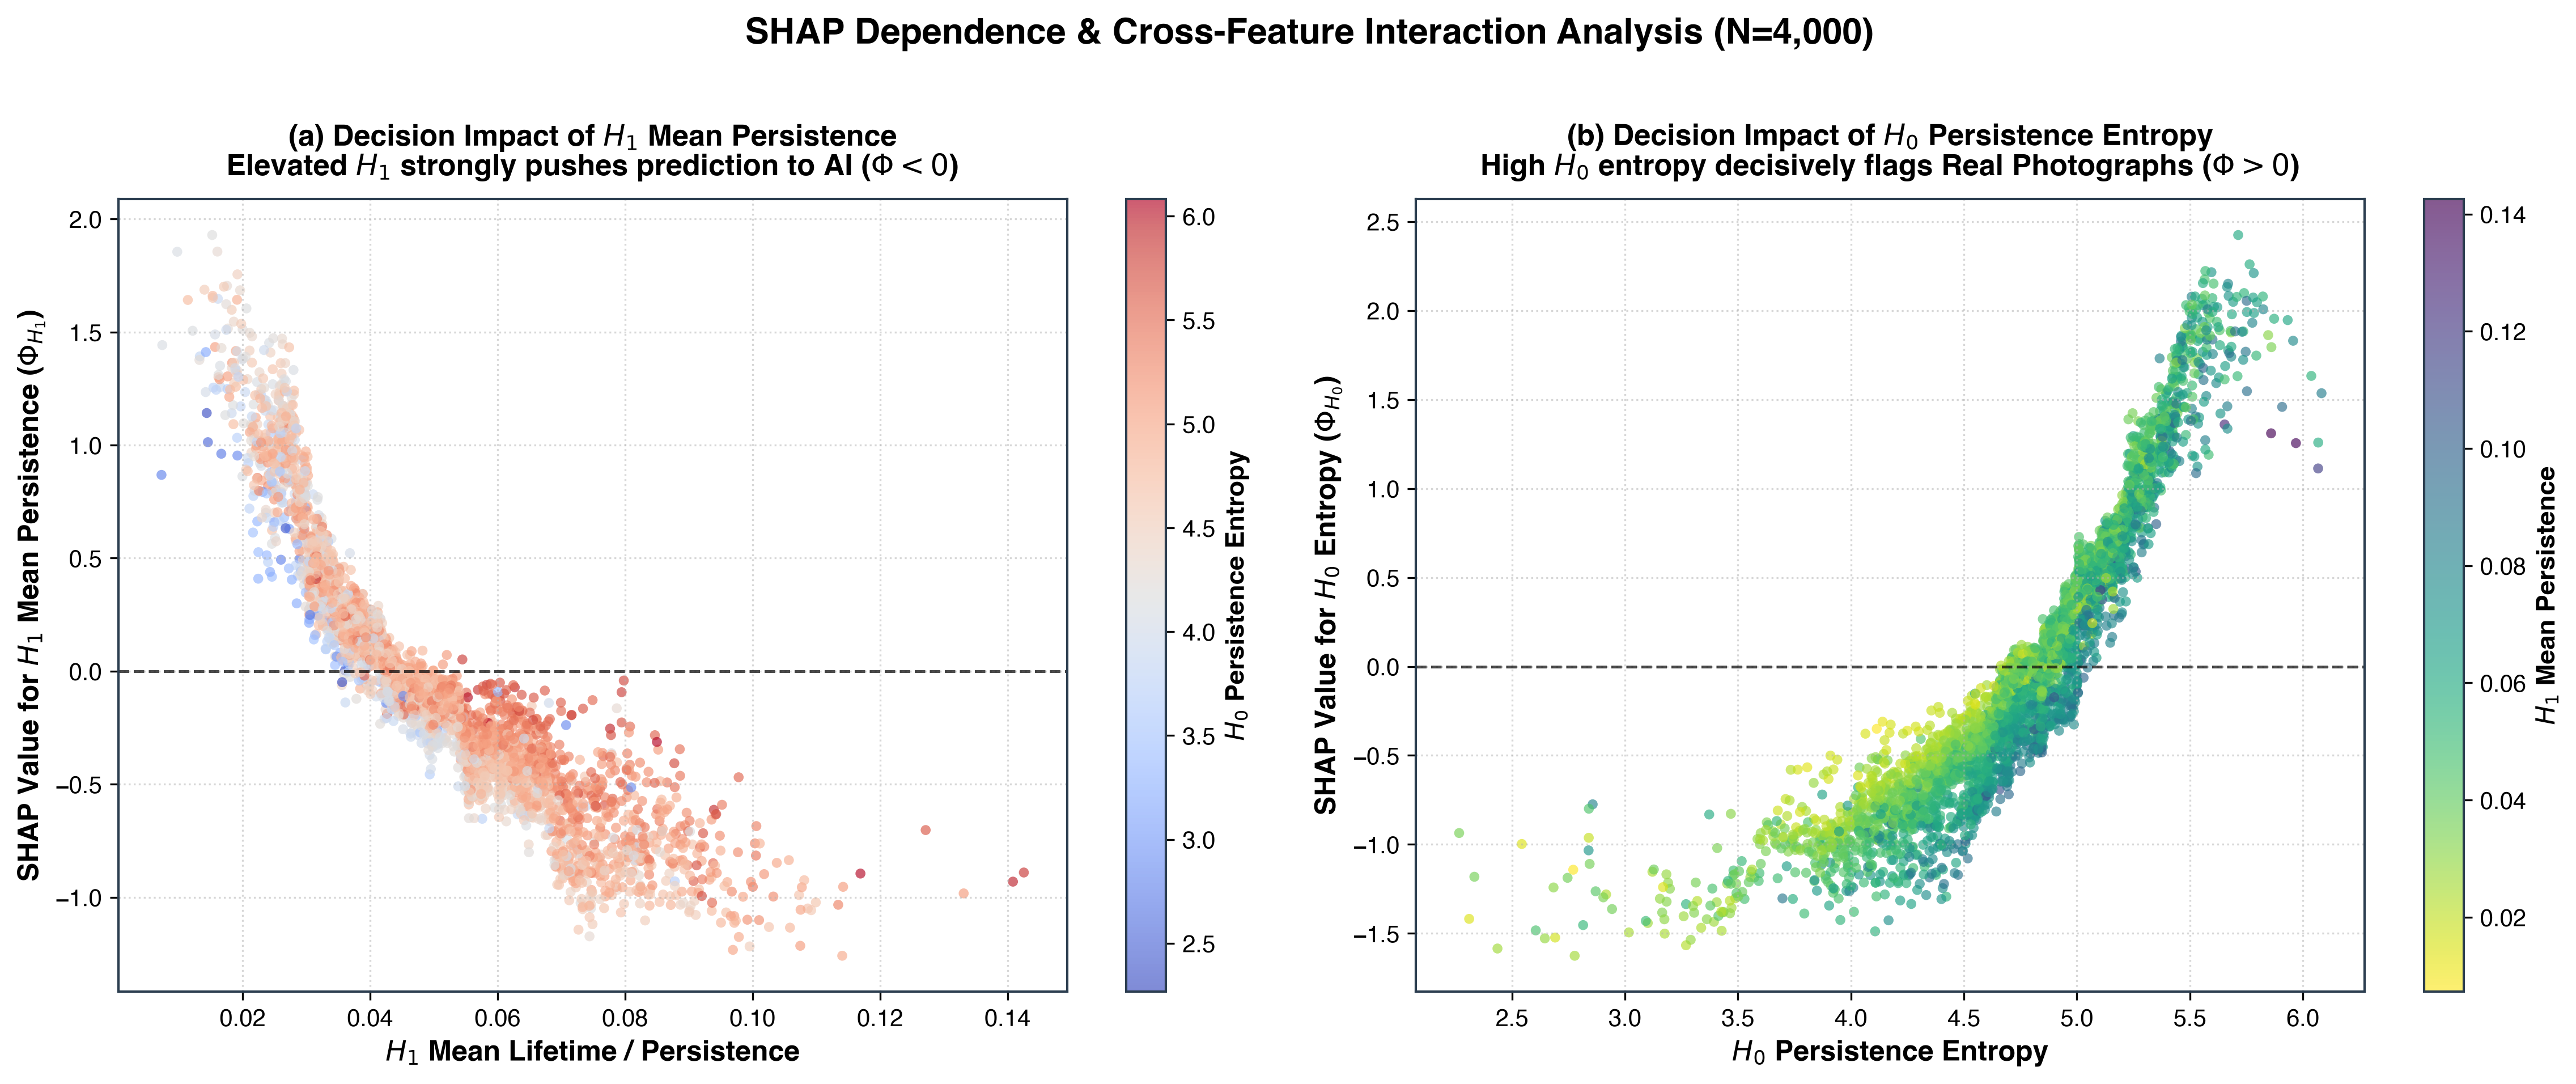
\includegraphics[width=\textwidth]{figures/shap_dependence_h1_mean_h0_entropy.png}
    \caption{SHAP dependence plots with cross-feature coloring for $H_1$ mean persistence (left) and $H_0$ persistence entropy (right) across $N=4{,}000$ test images.}
    \label{fig:shap_dependence}
\end{figure}

Figure~\ref{fig:shap_dependence} illustrates the dependence plots:
\begin{itemize}
    \item In panel (a), as $H_1$ mean persistence surpasses $0.050$, its attribution drops steeply into negative territory ($\Phi_{H_1} < 0$). Crucially, points with low $H_0$ entropy (blue scatter) experience an accelerated negative drop down to $\Phi_{H_1} \approx -1.5$, demonstrating compounding forensic evidence.
    \item In panel (b), $H_0$ persistence entropy exhibits a monotonic positive relationship with $\Phi_{H_0}$. Points with low $H_1$ persistence (dark purple scatter) attain the highest positive attributions ($\Phi_{H_0} > +1.5$).
\end{itemize}

\begin{figure}[H]
    \centering
    \begin{subfigure}[b]{0.48\textwidth}
        \centering
        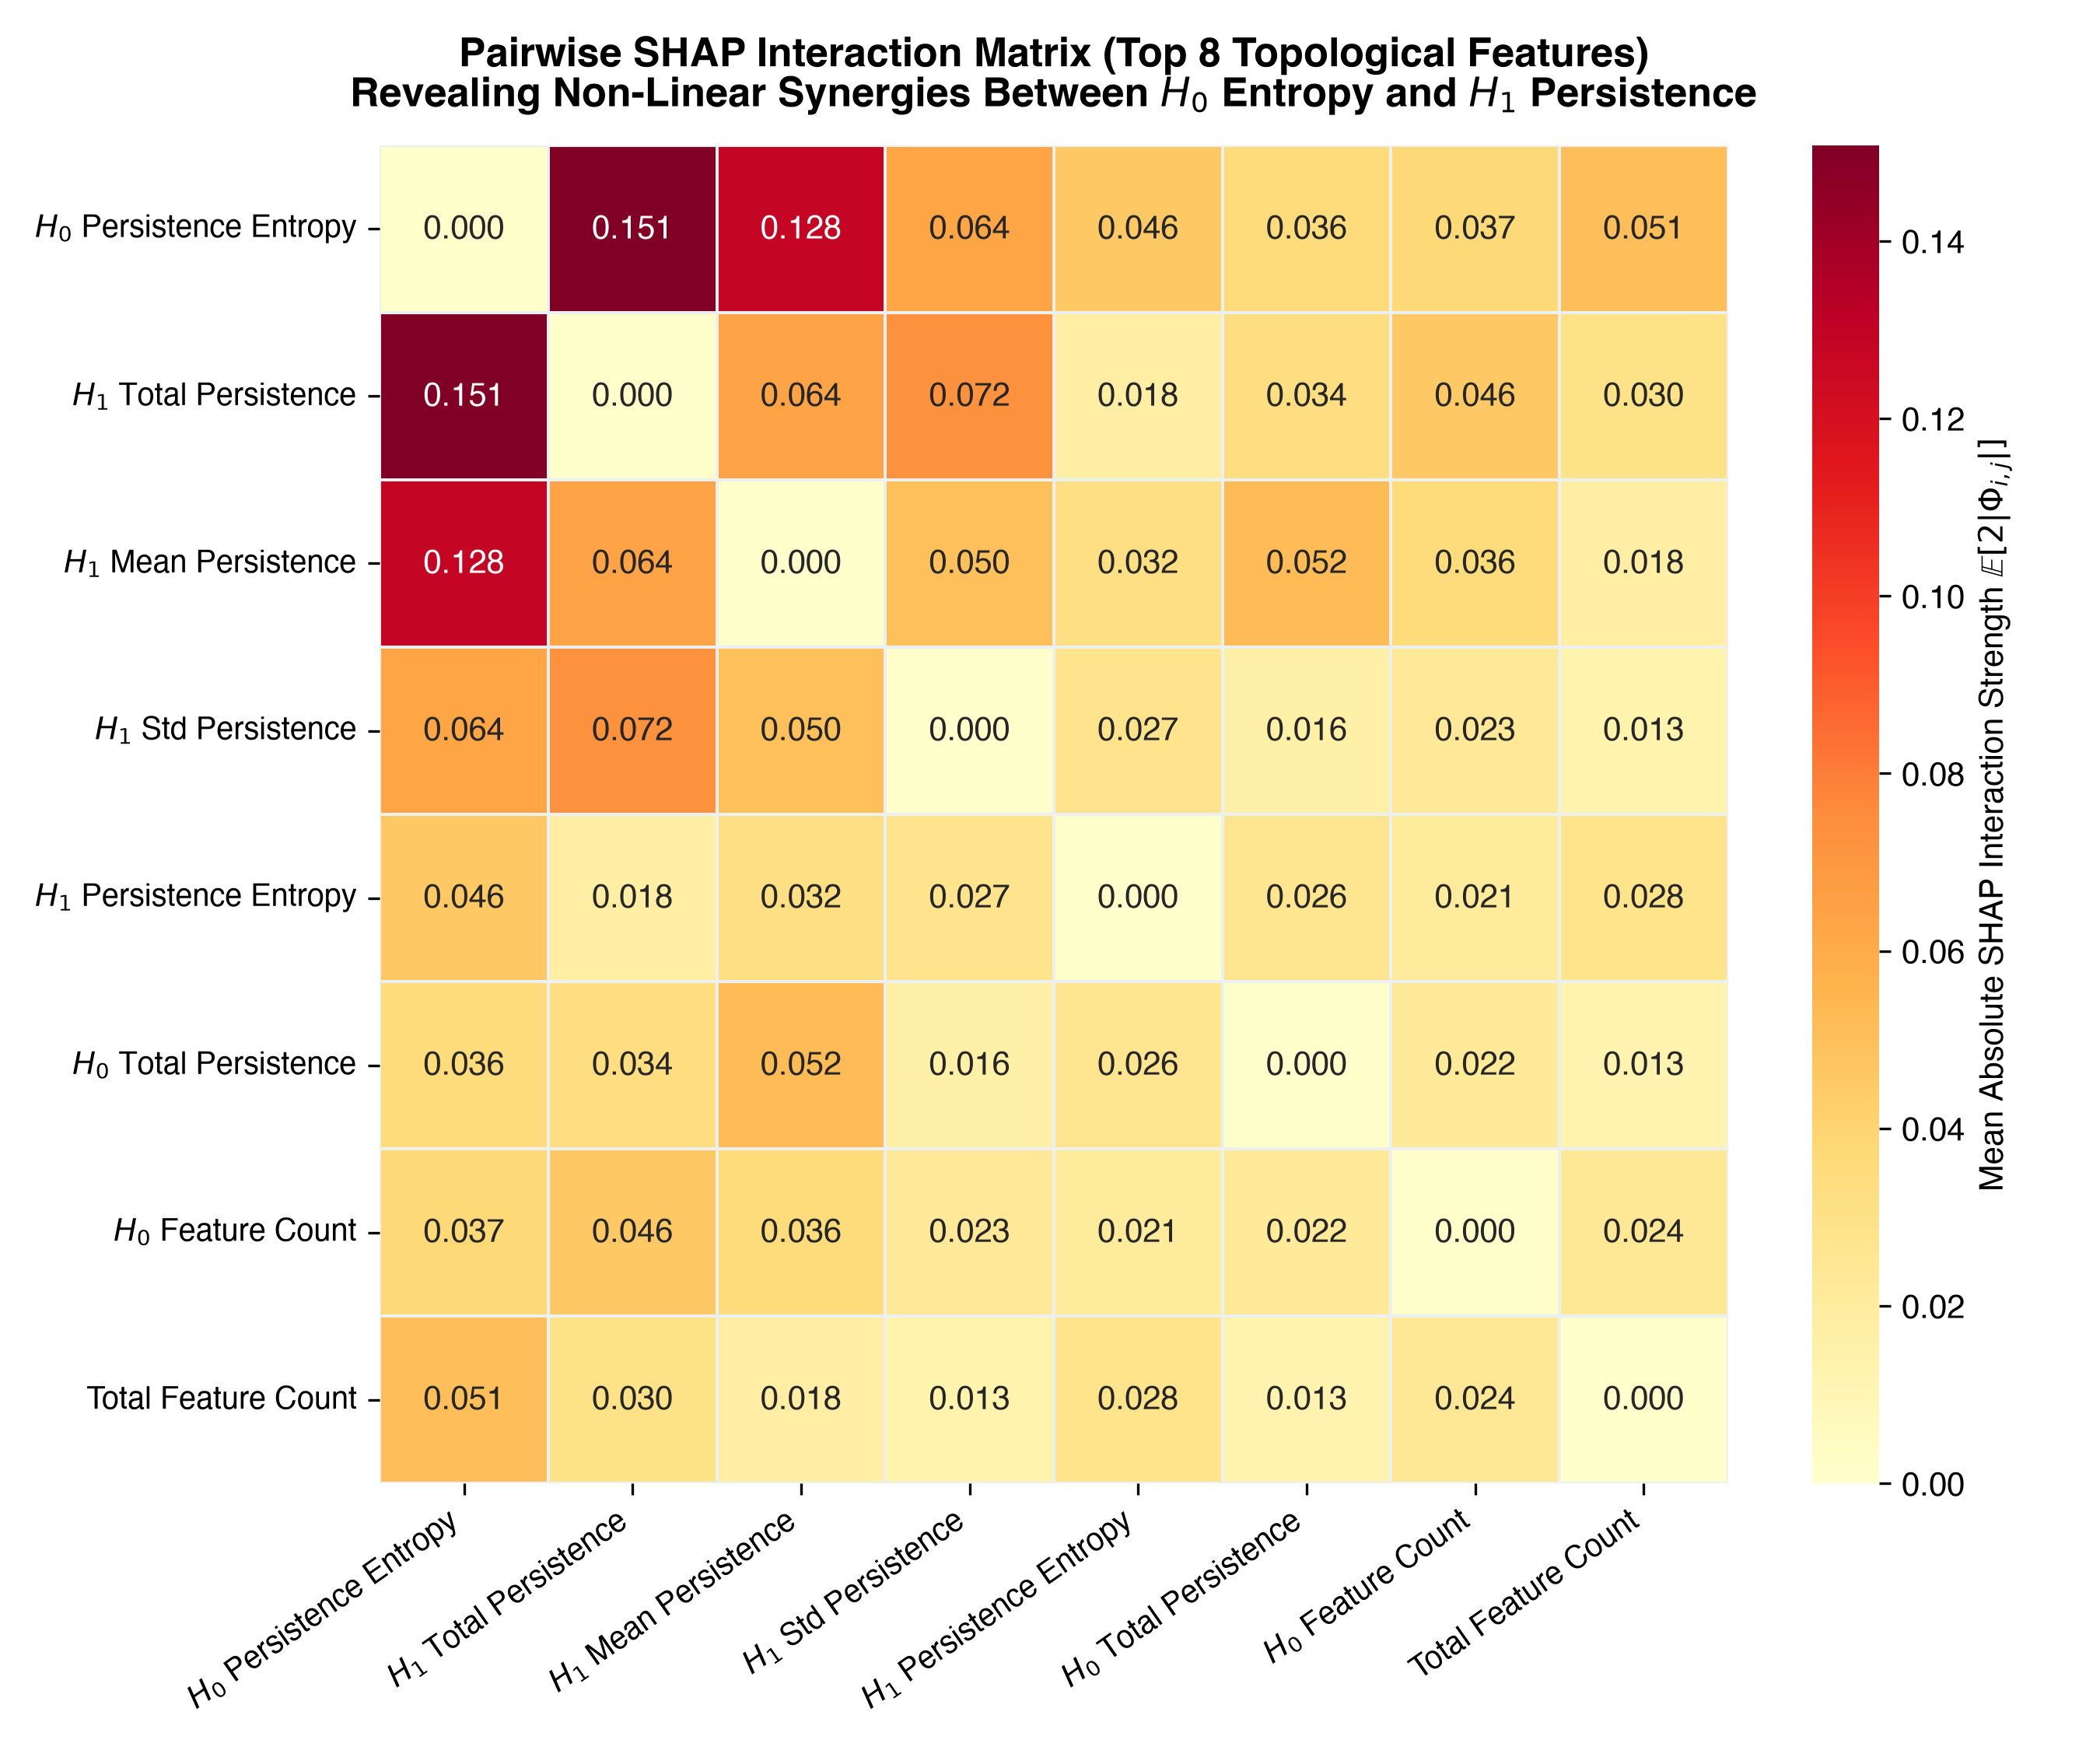
\includegraphics[width=\textwidth]{figures/shap_interaction_heatmap.png}
        \caption{Pairwise SHAP interaction matrix.}
        \label{fig:shap_heatmap}
    \end{subfigure}
    \hfill
    \begin{subfigure}[b]{0.48\textwidth}
        \centering
        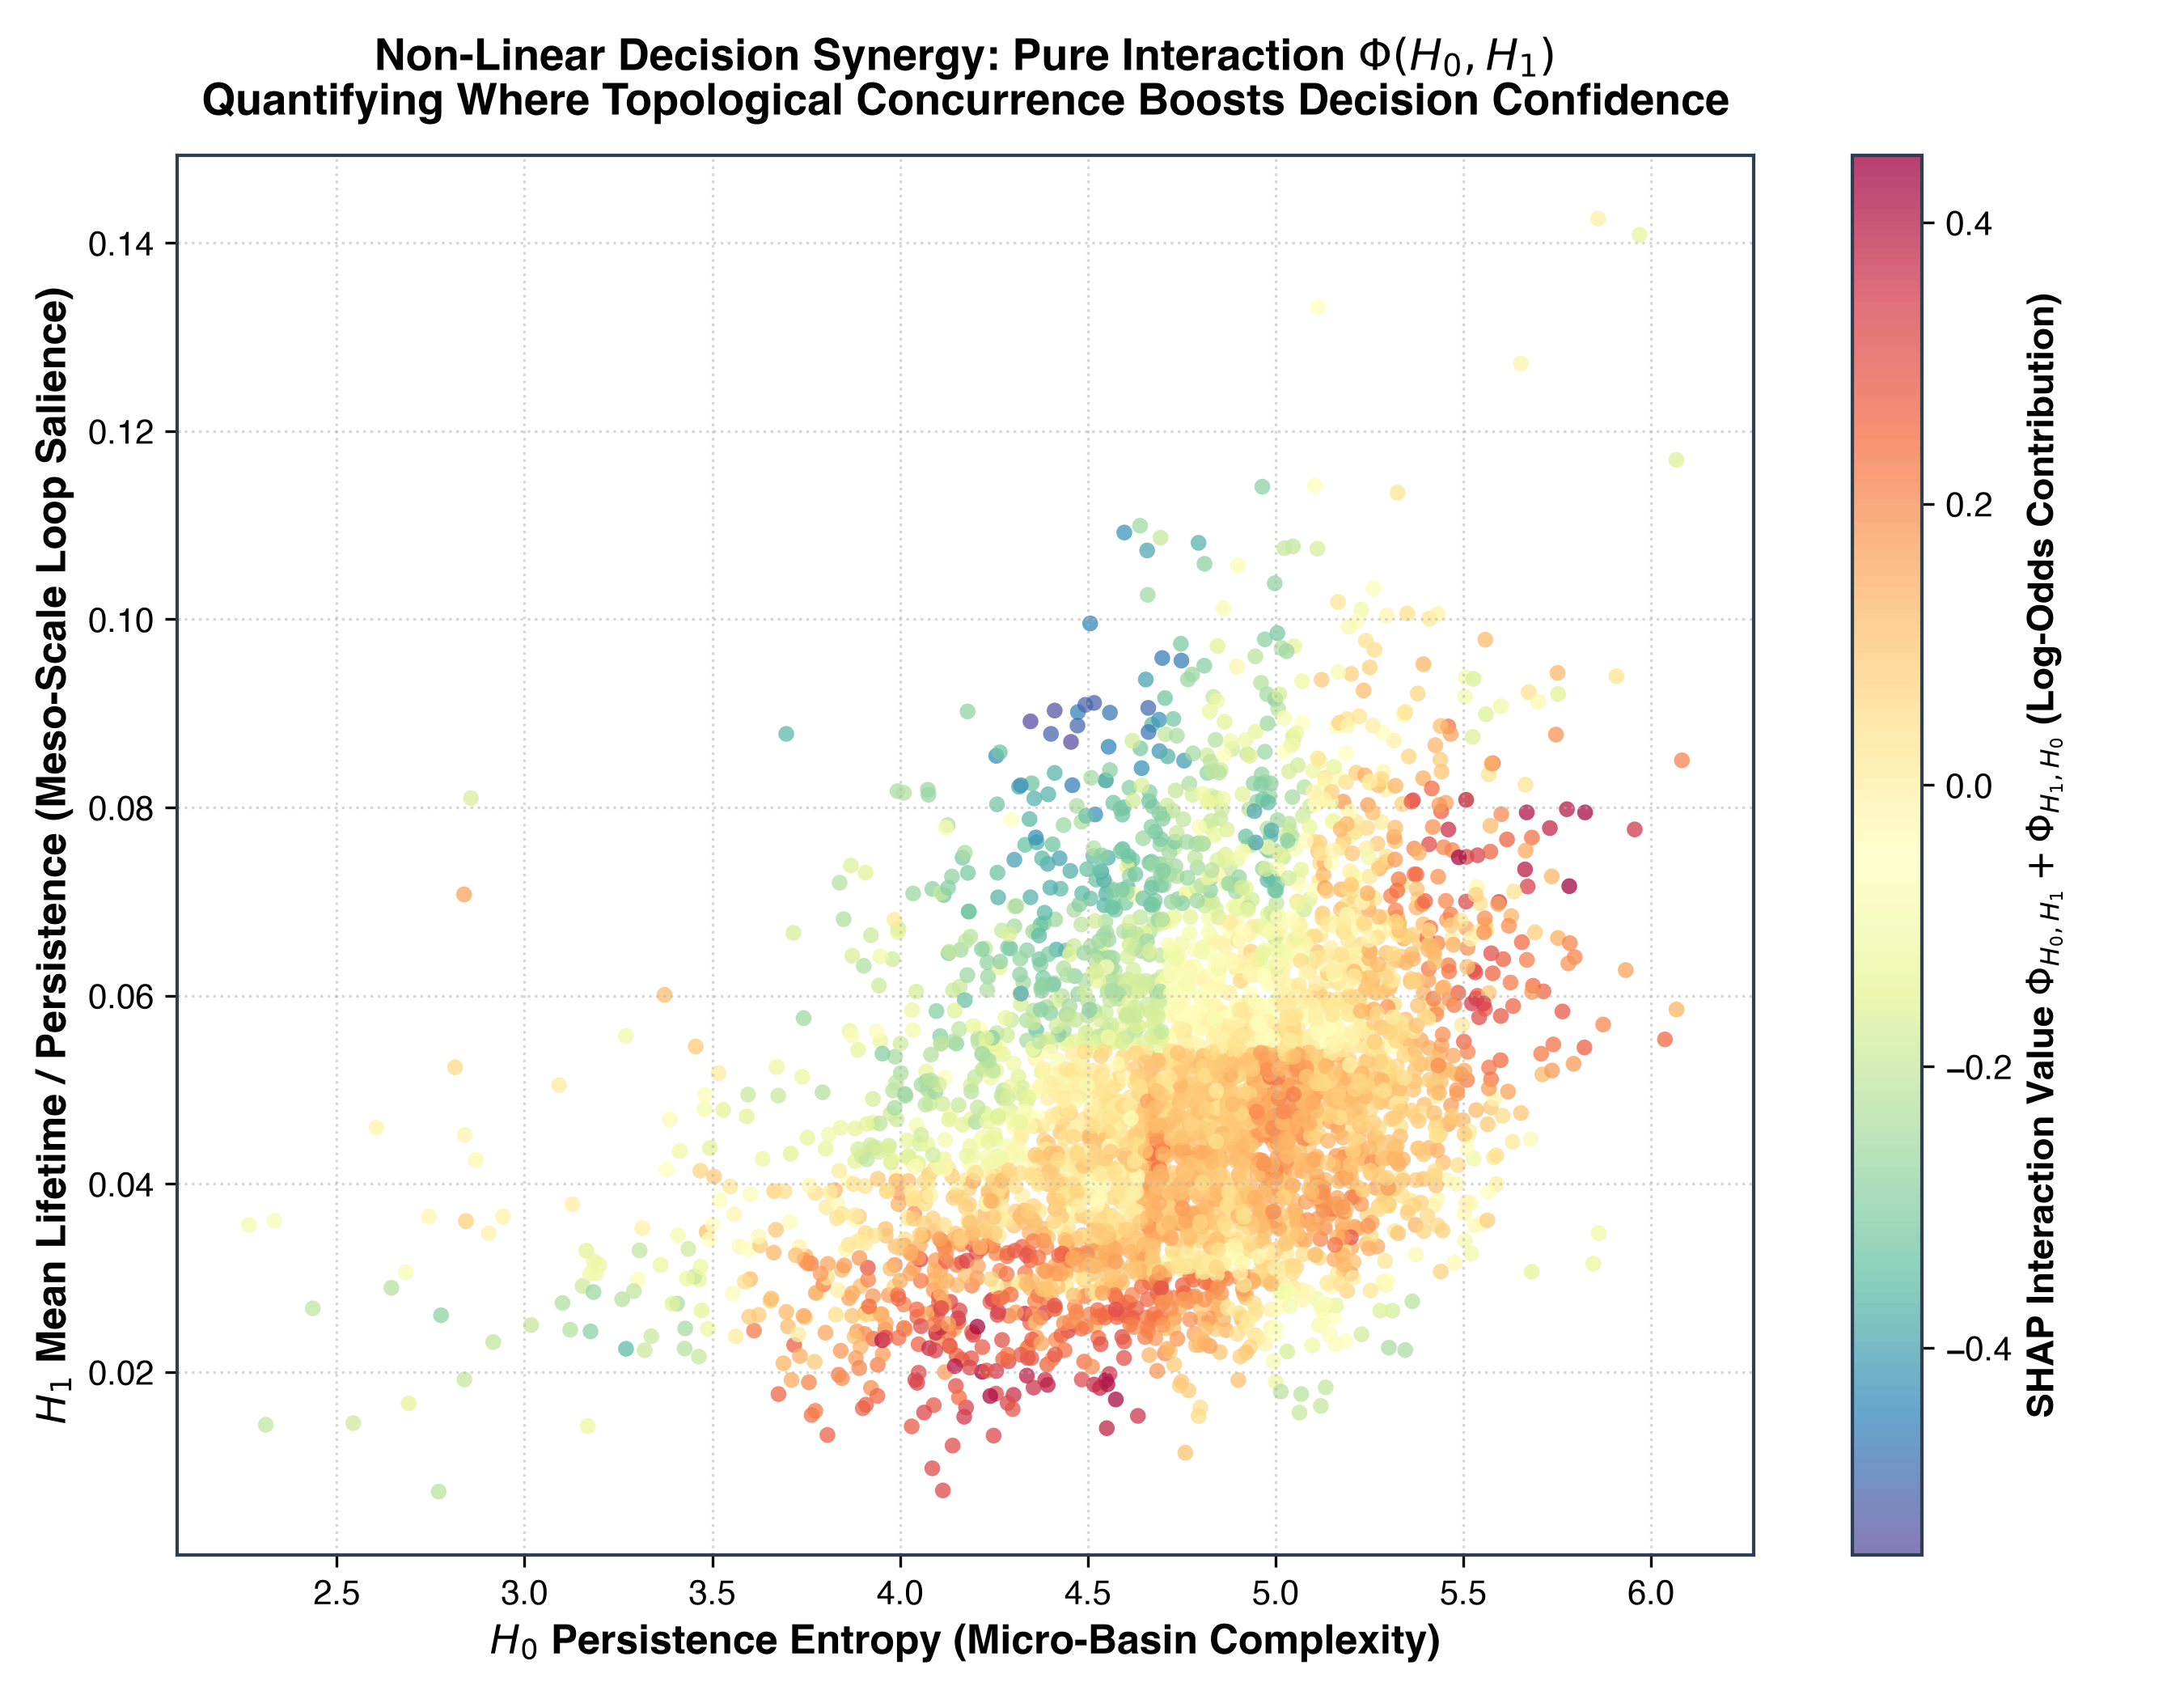
\includegraphics[width=\textwidth]{figures/shap_interaction_phase_space.png}
        \caption{Pure interaction $\Phi(H_0, H_1)$ in phase space.}
        \label{fig:shap_phase_scatter}
    \end{subfigure}
    \caption{Quantifying non-linear topological interactions: (a) pairwise interaction matrix among top 8 descriptors highlighting dominant $H_0 \times H_1$ synergies, and (b) pure interaction values mapped over the 2D topological phase space.}
    \label{fig:shap_interactions}
\end{figure}

As shown in Figure~\ref{fig:shap_interactions}(a), the pairwise interaction between $H_1$ total persistence and $H_0$ entropy exhibits the highest interaction energy across the entire model ($0.1508$), followed by $(H_0 \text{ entropy}, H_1 \text{ mean persistence})$ with $0.1282$. In Figure~\ref{fig:shap_interactions}(b), the pure interaction term is strongly active precisely along the boundary separating the real and AI clusters, illustrating an interaction in the fitted model. SHAP attributions and interactions describe predictions; they do not identify causal mechanisms or fractions of accuracy.

% ==============================================================================
\section{Continuous 2D Persistence Images and Deep Topological Learning}
% ==============================================================================

While the 16 scalar summary descriptors extract informative statistical moments, collapsing entire multi-scale persistence diagrams into single scalars inevitably discards rich geometric information regarding birth-death clustering, multi-modal distributions, and localized spatial correlations. To overcome this limitation, we extend our topological forensic framework to continuous two-dimensional \textbf{Persistence Images} (PI)~\cite{adams2017persistence} and evaluate a lightweight 2D Convolutional Neural Network (\textbf{TopoCNN}).

\subsection{Mathematical Formulation: From Diagrams to Continuous 2D Surfaces}
Let $\mathcal{D} = \{ (b_i, d_i) \}_{i=1}^n$ denote a persistence diagram in birth-death coordinates. We first apply the invertible linear transformation $T: (b, d) \mapsto (b, \ell = d - b)$ mapping each persistence pair to its birth-lifetime representation. 

A continuous persistence surface $\rho_{\mathcal{D}}(x, y)$ is defined over $\mathbb{R}^2$ as a weighted sum of normalized bivariate Gaussian kernels centered at each transformed point:
\begin{equation}
    \rho_{\mathcal{D}}(x, y) = \sum_{(b, \ell) \in T(\mathcal{D})} w(b, \ell) \, \frac{1}{2\pi \sigma^2} \exp\left( -\frac{(x - b)^2 + (y - \ell)^2}{2\sigma^2} \right)
\end{equation}
where $w(b, \ell)$ is a non-negative weighting function and $\sigma > 0$ is the Gaussian kernel bandwidth. To ensure that topological noise near the diagonal ($\ell \to 0$) does not dominate the representation, following the weighting principle of persistence images~\cite{adams2017persistence}, we employ the canonical linear lifetime weighting function:
\begin{equation}
    w(b, \ell) = \ell, \quad \ell > 0
\end{equation}

The implementation evaluates this surface at the points of a uniform $32\times32$ grid on $\Omega=[0,1]\times[0,1]$, with bandwidth $\sigma=0.05$. It does not integrate over cells or multiply by cell area. Thus the tensors used for the saved results are sampled persistence surfaces, although the code and historical figure labels call them persistence images. The standard cell-integrated construction of Adams et al. is a related but different representation. Lifetime weights are bounded here because normalized intensities give $0\le\ell\le1$.

For each image, this transformation is applied independently to zeroth-dimensional homology ($H_0$, connected components and intensity valleys) and first-dimensional homology ($H_1$, 1-cycles and peaks). Stacking both topological surfaces yields a two-channel tensor:
\begin{equation}
    \mathbf{X} \in \mathbb{R}^{2 \times 32 \times 32}, \quad \mathbf{X}[0, \cdot, \cdot] = \mathrm{PI}(H_0), \quad \mathbf{X}[1, \cdot, \cdot] = \mathrm{PI}(H_1)
\end{equation}

We process the complete 20,000-image CIFAKE evaluation partition using multi-core chunked parallelism, serializing the resulting topological data into two synchronized formats:
\begin{enumerate}[noitemsep]
    \item \textbf{Apache Parquet Dataset} (\path{data/cifake_persistence_dataset.parquet}): Structured table (144.2 MB) containing metadata, sample IDs, class labels, raw coordinate lists of $H_0$ and $H_1$ persistence pairs, and flattened persistence image arrays.
    \item \textbf{Compressed Tensor Archive} (\path{data/cifake_persistence_tensors.npz}): Packed float32 arrays (139.0 MB) of shape $(20{,}000, 2, 32, 32)$ ready for tensor ingestion by deep learning frameworks.
\end{enumerate}

\subsection{Topological Density Diagnostics: Real vs. AI Signatures}
Figure~\ref{fig:pi_diagnostics} illustrates the empirical mean persistence images across all 10,000 real photographs and 10,000 AI-generated images, together with differential density surfaces ($\Delta = \text{AI} - \text{Real}$) and sample diagrams.

\begin{figure}[H]
    \centering
    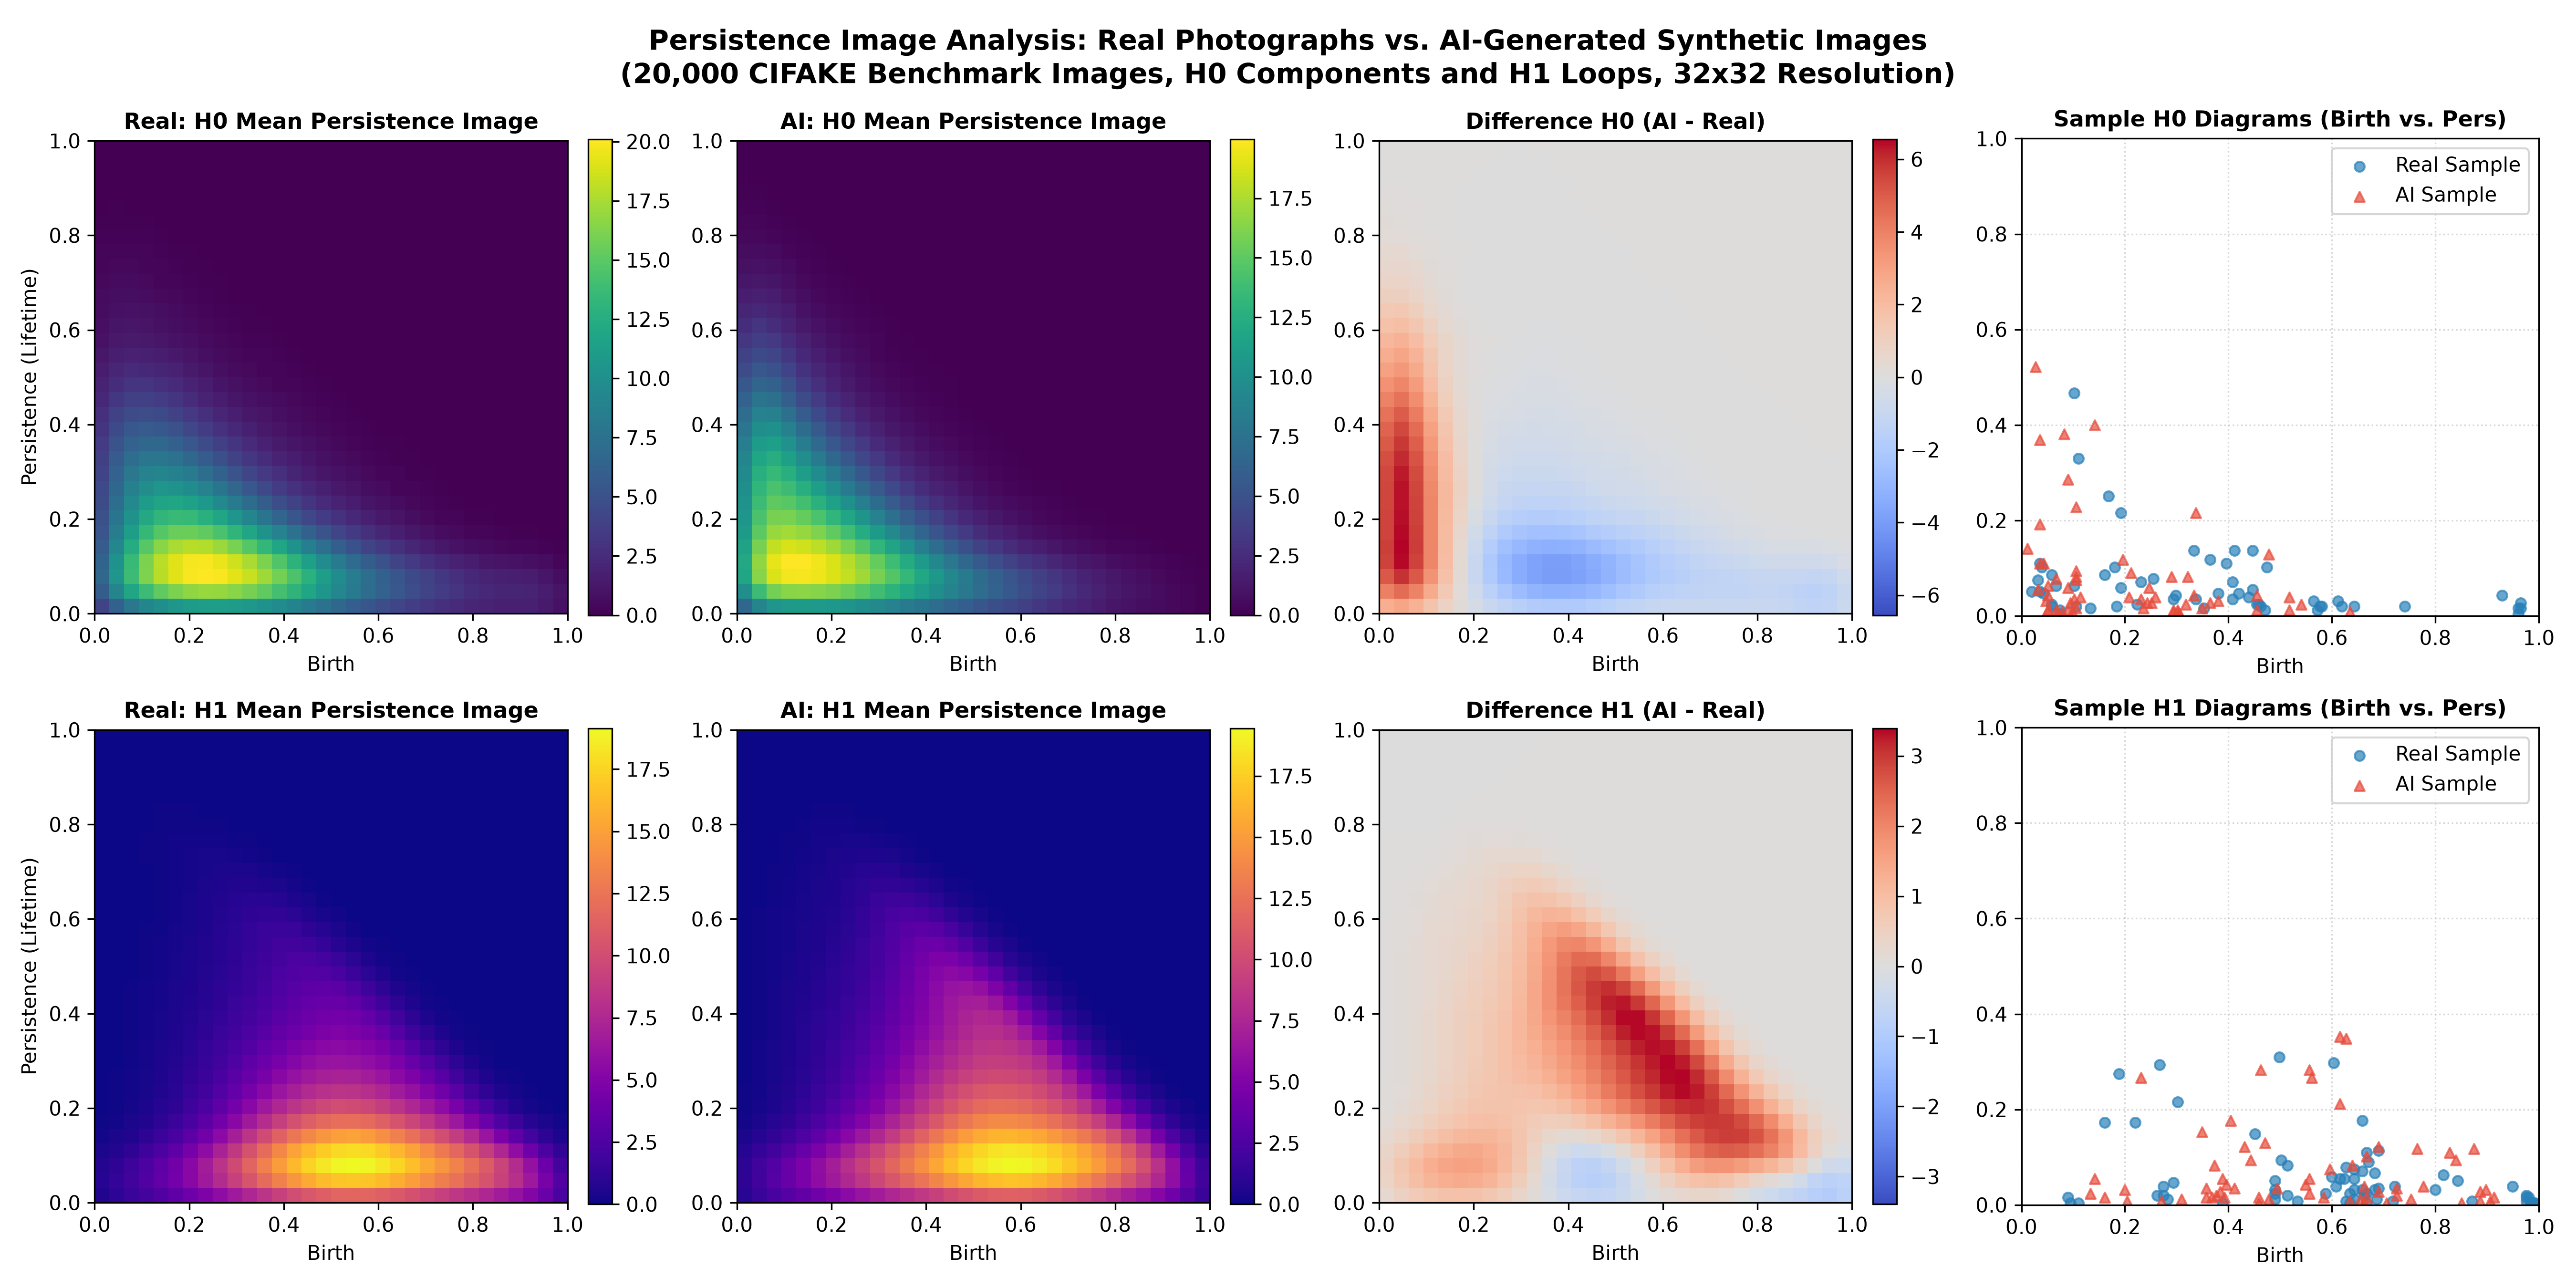
\includegraphics[width=\textwidth]{figures/persistence_images_samples.png}
    \caption{Persistence Image analysis across 20,000 CIFAKE images ($32 \times 32$ resolution, bandwidth $\sigma=0.05$, lifetime weighting $w(\ell)=\ell$). Top row: $H_0$ connected components. Bottom row: $H_1$ topological loops. The third column displays differential density maps ($\text{AI} - \text{Real}$); the fourth column illustrates sample persistence diagrams in birth-lifetime coordinates.}
    \label{fig:pi_diagnostics}
\end{figure}

The continuous density maps reveal distinct structural characteristics:
\begin{itemize}
    \item \textbf{$H_0$ Homology (Intensity Valleys)}: Physical photographs exhibit a uniform, broad horizontal density band along the low-lifetime baseline ($\ell \in [0.01, 0.05]$) spanning the entire birth interval $[0.0, 1.0]$. This records short-lived intensity features; attributing them to photon noise or sensor grain would require controlled experiments. Conversely, AI images display lower density in this low-persistence regime, as reflected by negative values in the difference map.
    \item \textbf{$H_1$ Homology (Topological Loops)}: Stable Diffusion images concentrate significantly higher density in intermediate and high persistence ($\ell \in [0.06, 0.20]$), clearly evidenced by the intense red cluster in the difference map ($\Delta > 0$). This records differences in the persistence distribution, without identifying a specific generative mechanism.
\end{itemize}

\subsection{Lightweight Deep Architecture: TopoCNN}
To leverage spatial correlations in birth-lifetime space without the computational overhead and overfitting risks of heavy vision backbones, we design \textbf{TopoCNN}, a compact 2D Convolutional Neural Network comprising only \textbf{122,914 trainable parameters}. The architecture is structured as follows:
\begin{enumerate}
    \item \textbf{Stem}: A $3 \times 3$ convolution projecting the $2$-channel topological input into $16$ feature maps, followed by Batch Normalization and Gaussian Error Linear Unit (GELU) activation~\cite{hendrycks2016gaussian}.
    \item \textbf{Stage 1}: A residual convolutional block maintaining $16$ channels at $32 \times 32$ spatial resolution.
    \item \textbf{Downsampling Stage 2}: A strided $3 \times 3$ convolution ($\text{stride}=2$) downsampling feature maps to $16 \times 16$ with $32$ channels, followed by a 32-channel residual block.
    \item \textbf{Downsampling Stage 3}: A second strided $3 \times 3$ convolution downsampling to $8 \times 8$ with $64$ channels, followed by a 64-channel residual block.
    \item \textbf{Global Pooling and Classifier Head}: Global Adaptive Average Pooling compresses the spatial dimensions to a 64-dimensional latent topological vector. A regularized two-layer classification head ($\text{Dropout}(0.3) \to \text{Linear}(64, 32) \to \text{GELU} \to \text{Dropout}(0.2) \to \text{Linear}(32, 2)$) computes class logits.
\end{enumerate}

\paragraph{Training Protocol.}
The model is trained using the exact same stratified 80/20 partition ($N_{\text{train}} = 16{,}000$, $N_{\text{test}} = 4{,}000$, random seed 42) established in the baseline benchmark. Within the training set, a $10\%$ stratified split ($1{,}600$ images) serves as the validation monitor for selecting the best checkpoint. The code runs all 22 epochs; it does not implement early stopping. Training employs the AdamW optimizer ($\eta = 10^{-3}$, weight decay $10^{-4}$), a Cosine Annealing learning rate schedule ($\eta_{\min} = 10^{-5}$), batch size 64, and Cross-Entropy loss with $0.05$ label smoothing. Computations are executed via Apple Silicon Metal Performance Shaders (MPS), running 22 epochs in \textbf{75.6 seconds}.

\begin{figure}[H]
    \centering
    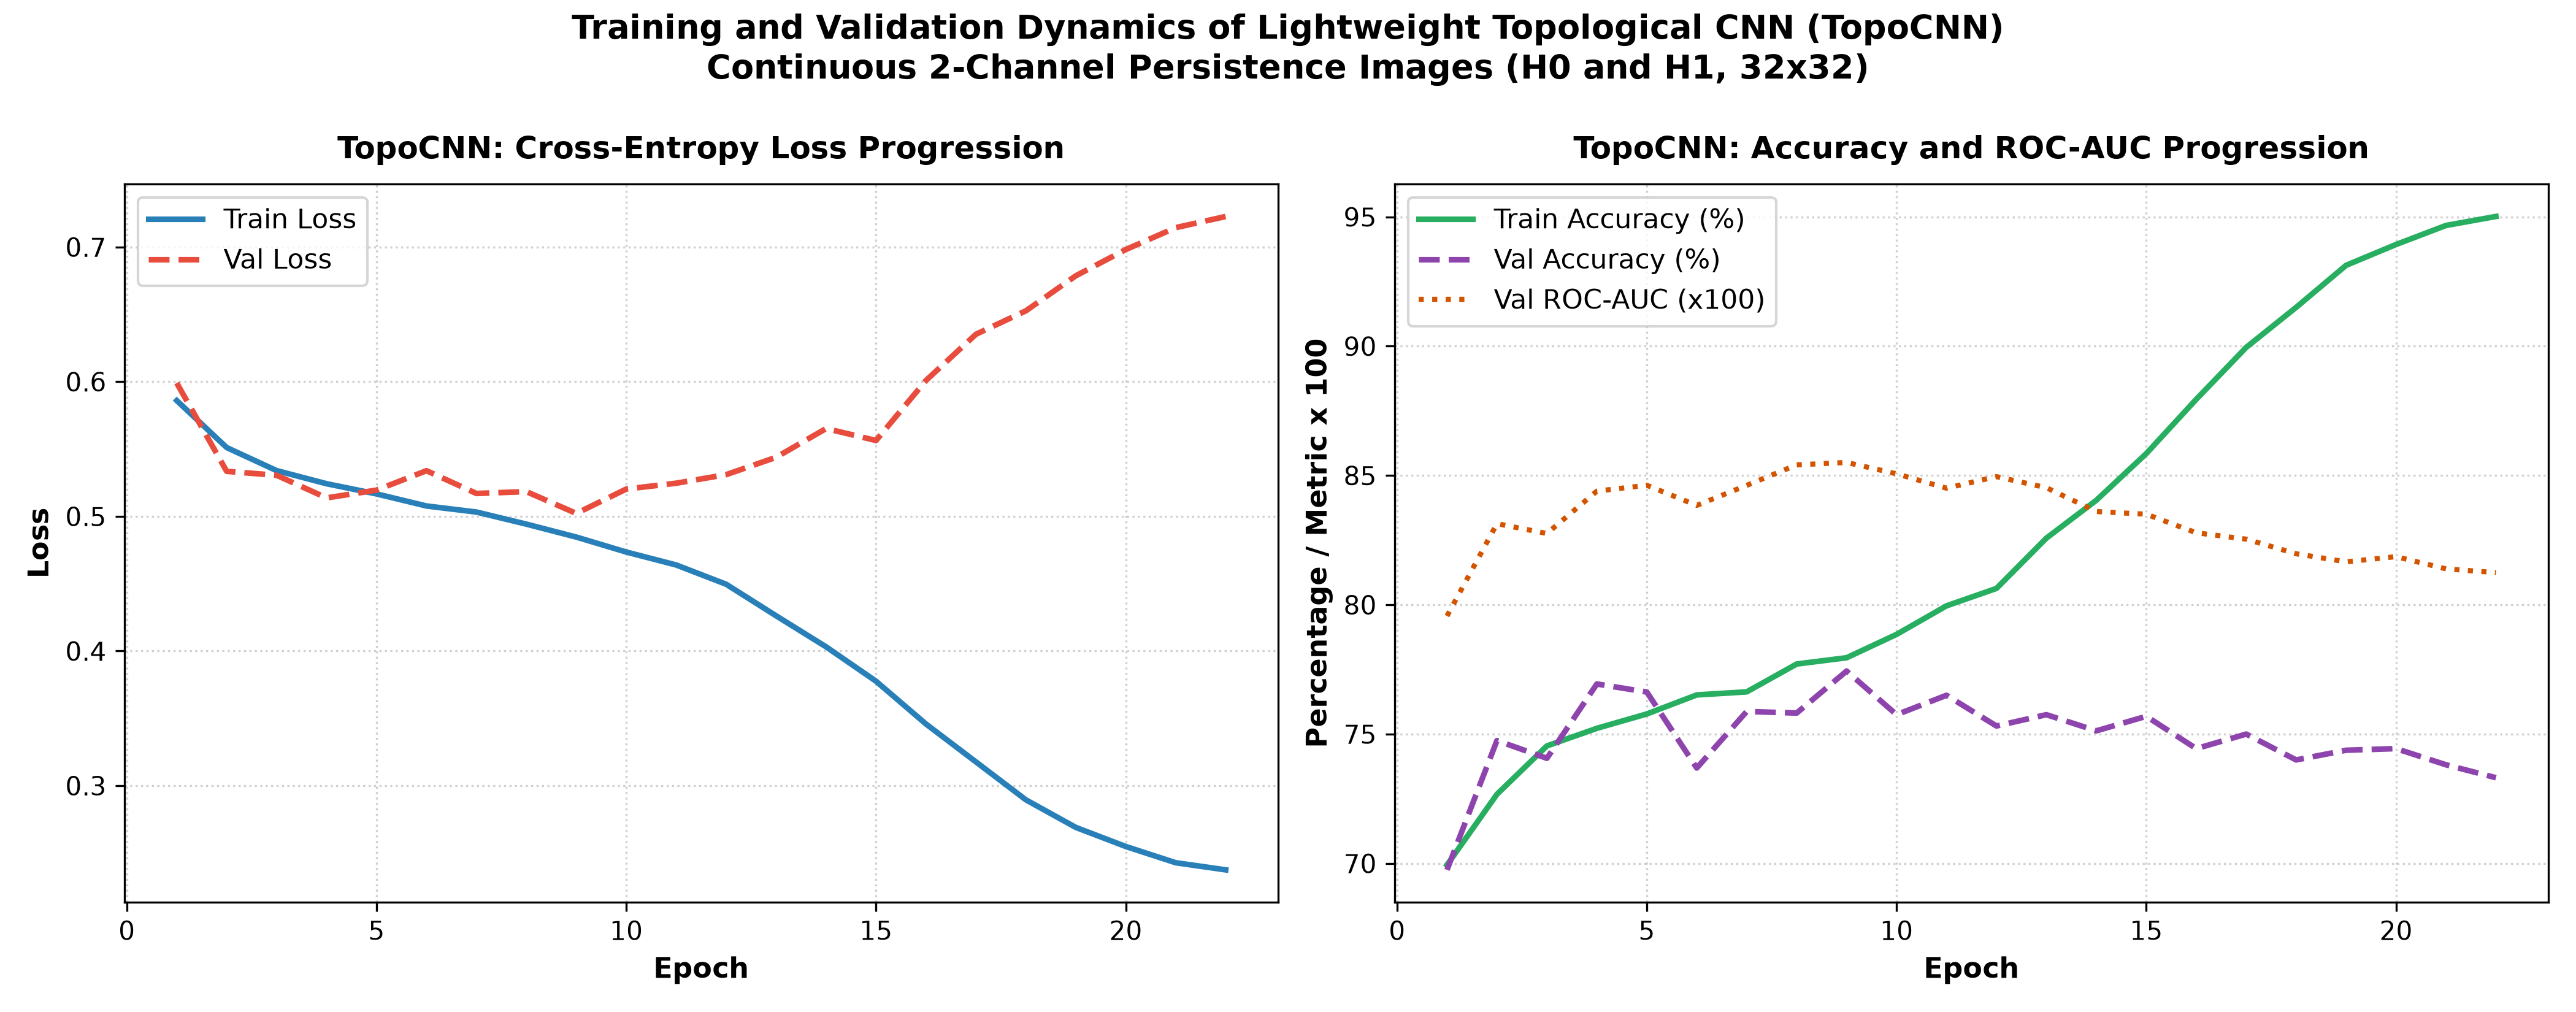
\includegraphics[width=0.92\textwidth]{figures/cnn_learning_curves.png}
    \caption{Training and validation dynamics of TopoCNN over 22 epochs on $2$-channel persistence images. Left: Cross-Entropy loss. Right: Classification accuracy and validation ROC-AUC.}
    \label{fig:cnn_curves}
\end{figure}

As shown in Figure~\ref{fig:cnn_curves}, the saved learning-curve figure reports a best validation ROC-AUC of \textbf{0.8550} at epoch 9, with the best model checkpoint preserved at \path{models/topo_cnn_best.pt}.

\subsection{Master Forensic Benchmark: Tabular Descriptors vs. 2D CNN}
Table~\ref{tab:master_benchmark} presents the comprehensive performance benchmark comparing all six tabular classifiers trained on 1D scalar descriptors against TopoCNN trained on 2D Persistence Images, evaluated on the identical $4{,}000$-image test split ($2{,}000$ Real vs. $2{,}000$ AI).

\begin{table}[H]
\centering
\small
\caption{Comprehensive Forensic Benchmark: 1D Topological Descriptors vs. 2D Persistence Images ($N_{\text{test}} = 4{,}000$).}
\label{tab:master_benchmark}
\resizebox{\textwidth}{!}{%
\begin{tabular}{llccccccc}
\toprule
\textbf{Model Architecture} & \textbf{Topological Input} & \textbf{Test Acc.} & \textbf{Balanced Acc.} & \textbf{Test AUC} & \textbf{Test F1} & \textbf{Precision} & \textbf{Recall} & \textbf{Brier Score} \\
\midrule
Logistic Regression (L2) & 16 Scalar Descriptors & $68.90\%$ & $68.90\%$ & $0.7646$ & $0.7018$ & $0.6740$ & $0.7320$ & $0.1969$ \\
Linear SVM & 16 Scalar Descriptors & $68.90\%$ & $68.90\%$ & $0.7644$ & $0.7015$ & $0.6744$ & $0.7310$ & $0.1970$ \\
Random Forest & 16 Scalar Descriptors & $69.55\%$ & $69.55\%$ & $0.7750$ & $0.7078$ & $0.6804$ & $0.7375$ & $0.1923$ \\
XGBoost & 16 Scalar Descriptors & $69.73\%$ & $69.73\%$ & $0.7756$ & $0.7074$ & $0.6844$ & $0.7320$ & $0.1924$ \\
LightGBM & 16 Scalar Descriptors & $69.95\%$ & $69.95\%$ & $0.7789$ & $0.7135$ & $0.6817$ & $0.7485$ & $0.1911$ \\
RBF SVM & 16 Scalar Descriptors & $70.03\%$ & $70.03\%$ & $0.7755$ & $0.7138$ & $0.6830$ & $0.7475$ & $0.1932$ \\
\midrule
\textbf{TopoCNN (Ours)} & \textbf{2D Persistence Images ($32 \times 32 \times 2$)} & $\mathbf{74.70\%}$ & $\mathbf{74.70\%}$ & $\mathbf{0.8404}$ & $\mathbf{0.7637}$ & $\mathbf{0.7165}$ & $\mathbf{0.8175}$ & $\mathbf{0.1657}$ \\
\bottomrule
\end{tabular}%
}
\end{table}

\begin{figure}[H]
    \centering
    \begin{subfigure}[b]{0.52\textwidth}
        \centering
        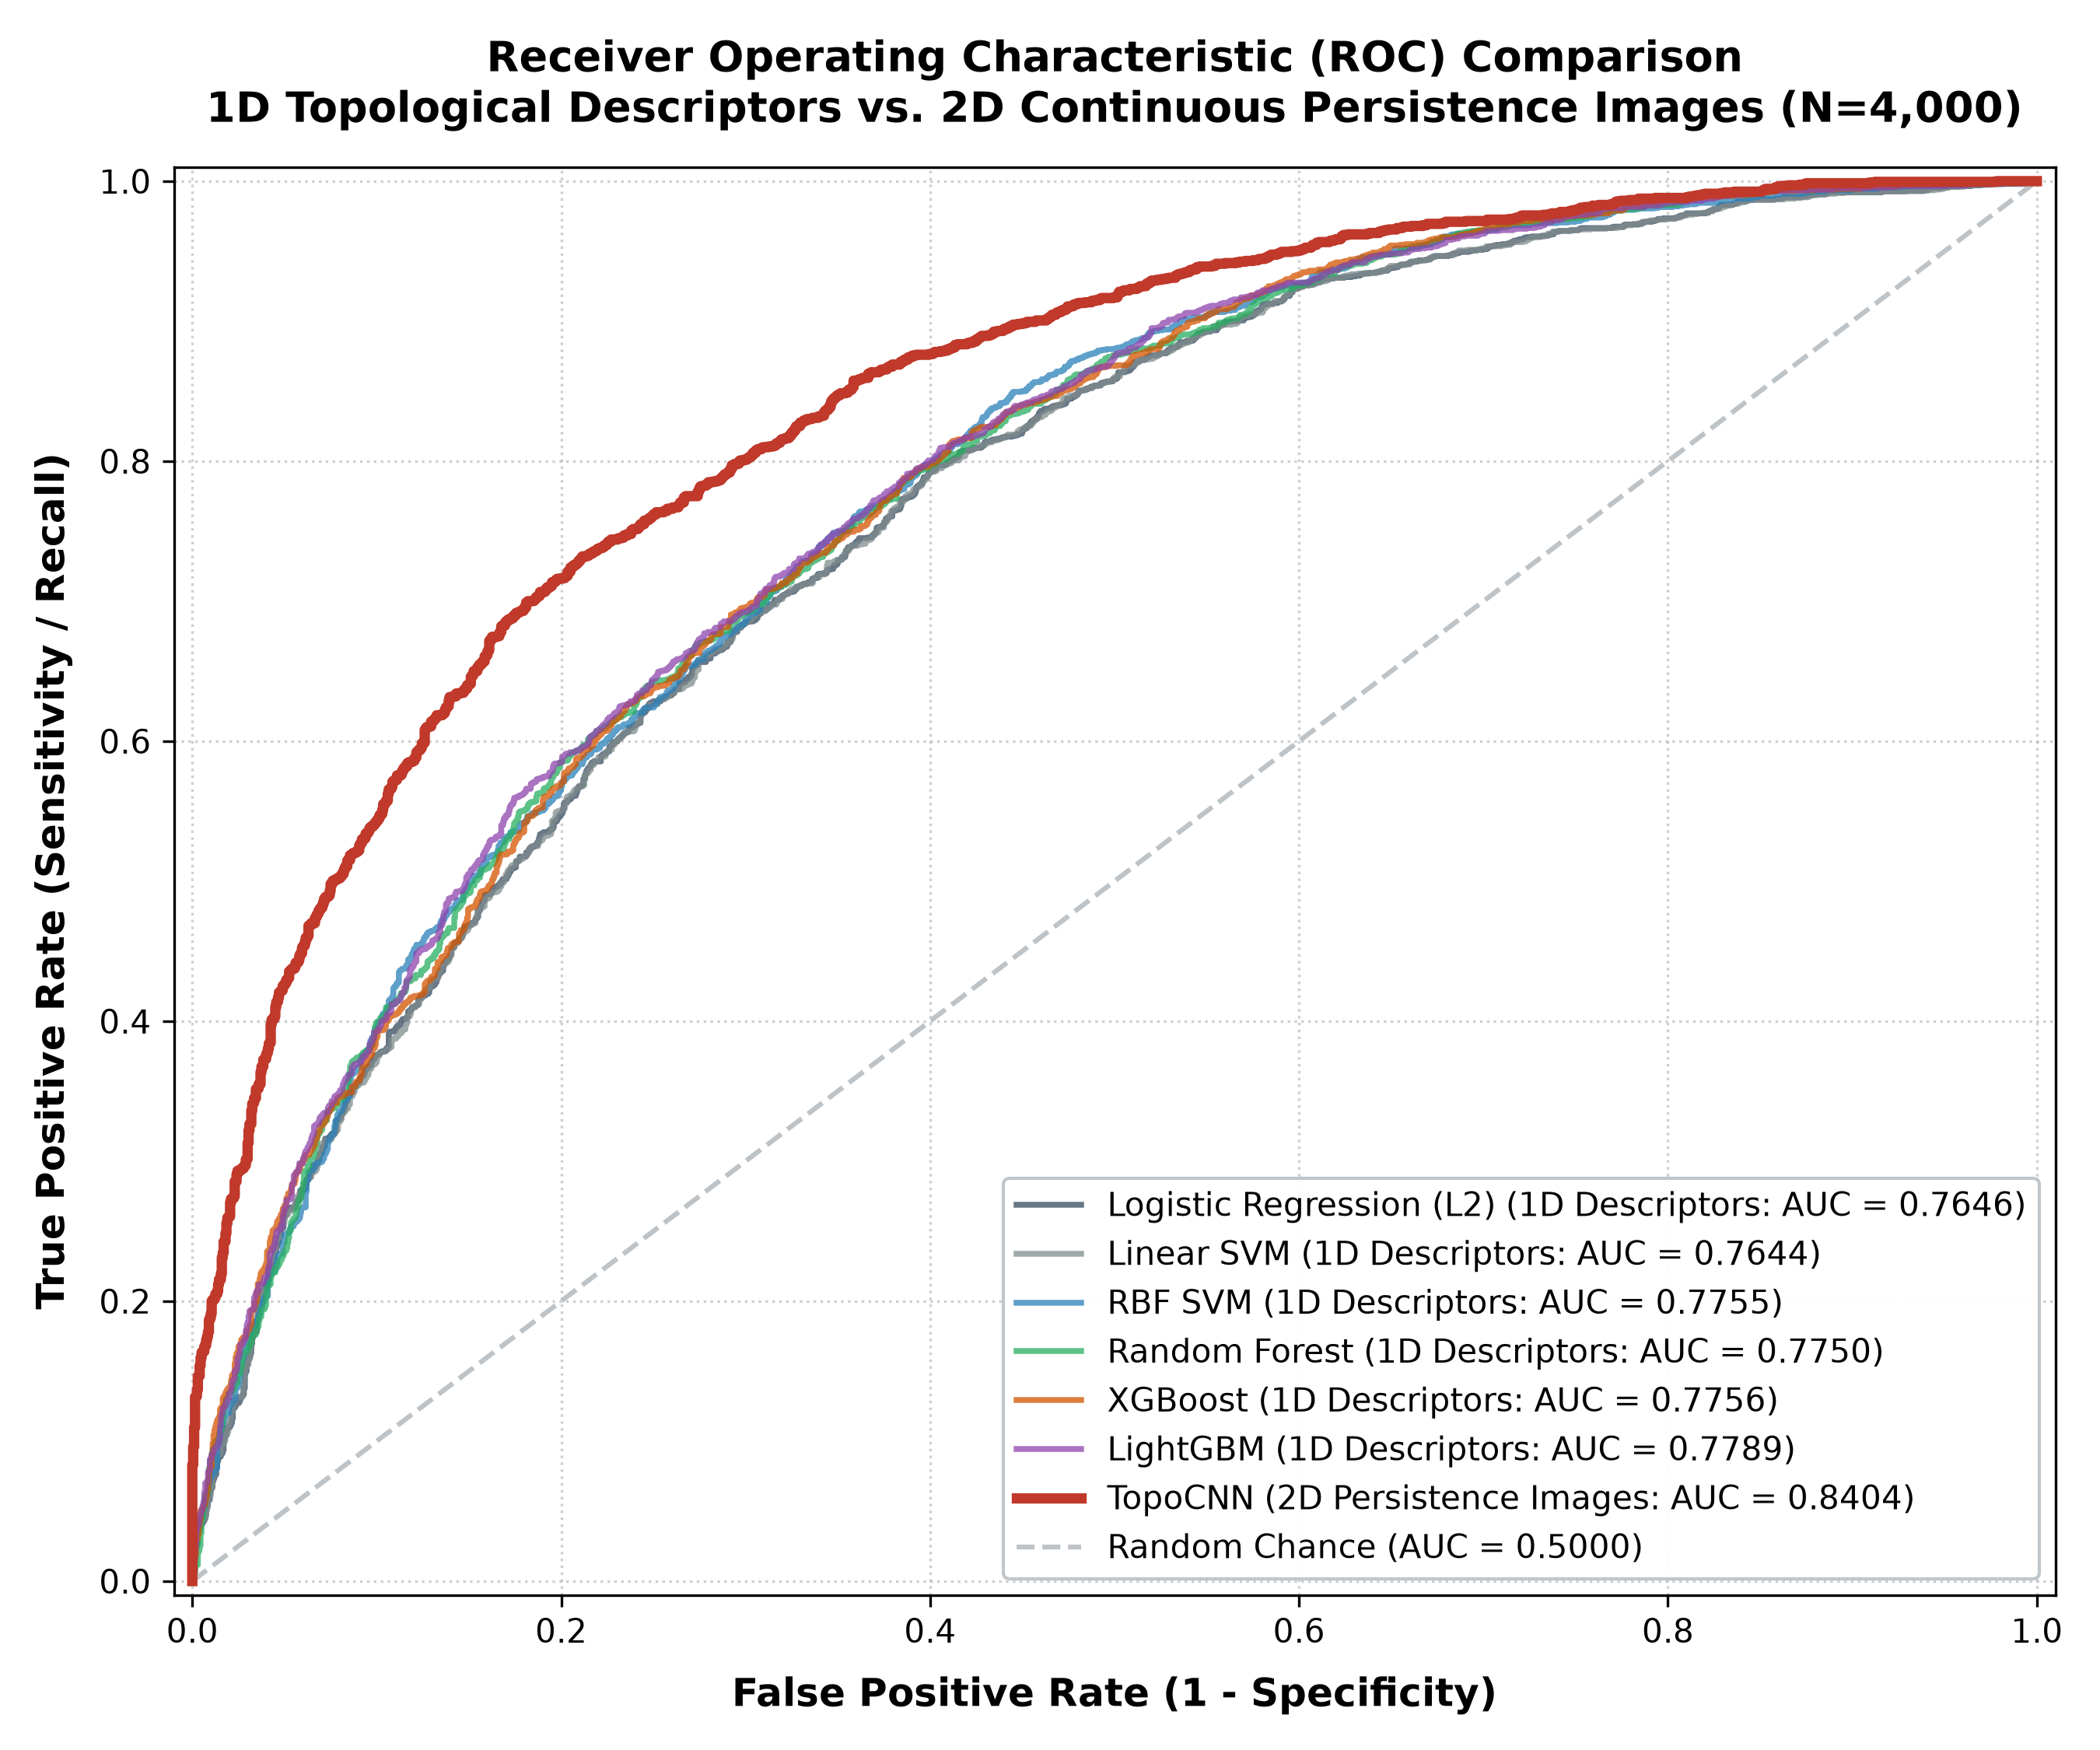
\includegraphics[width=\textwidth]{figures/roc_curves_with_cnn.png}
        \caption{Combined ROC benchmark comparison.}
        \label{fig:roc_with_cnn}
    \end{subfigure}
    \hfill
    \begin{subfigure}[b]{0.44\textwidth}
        \centering
        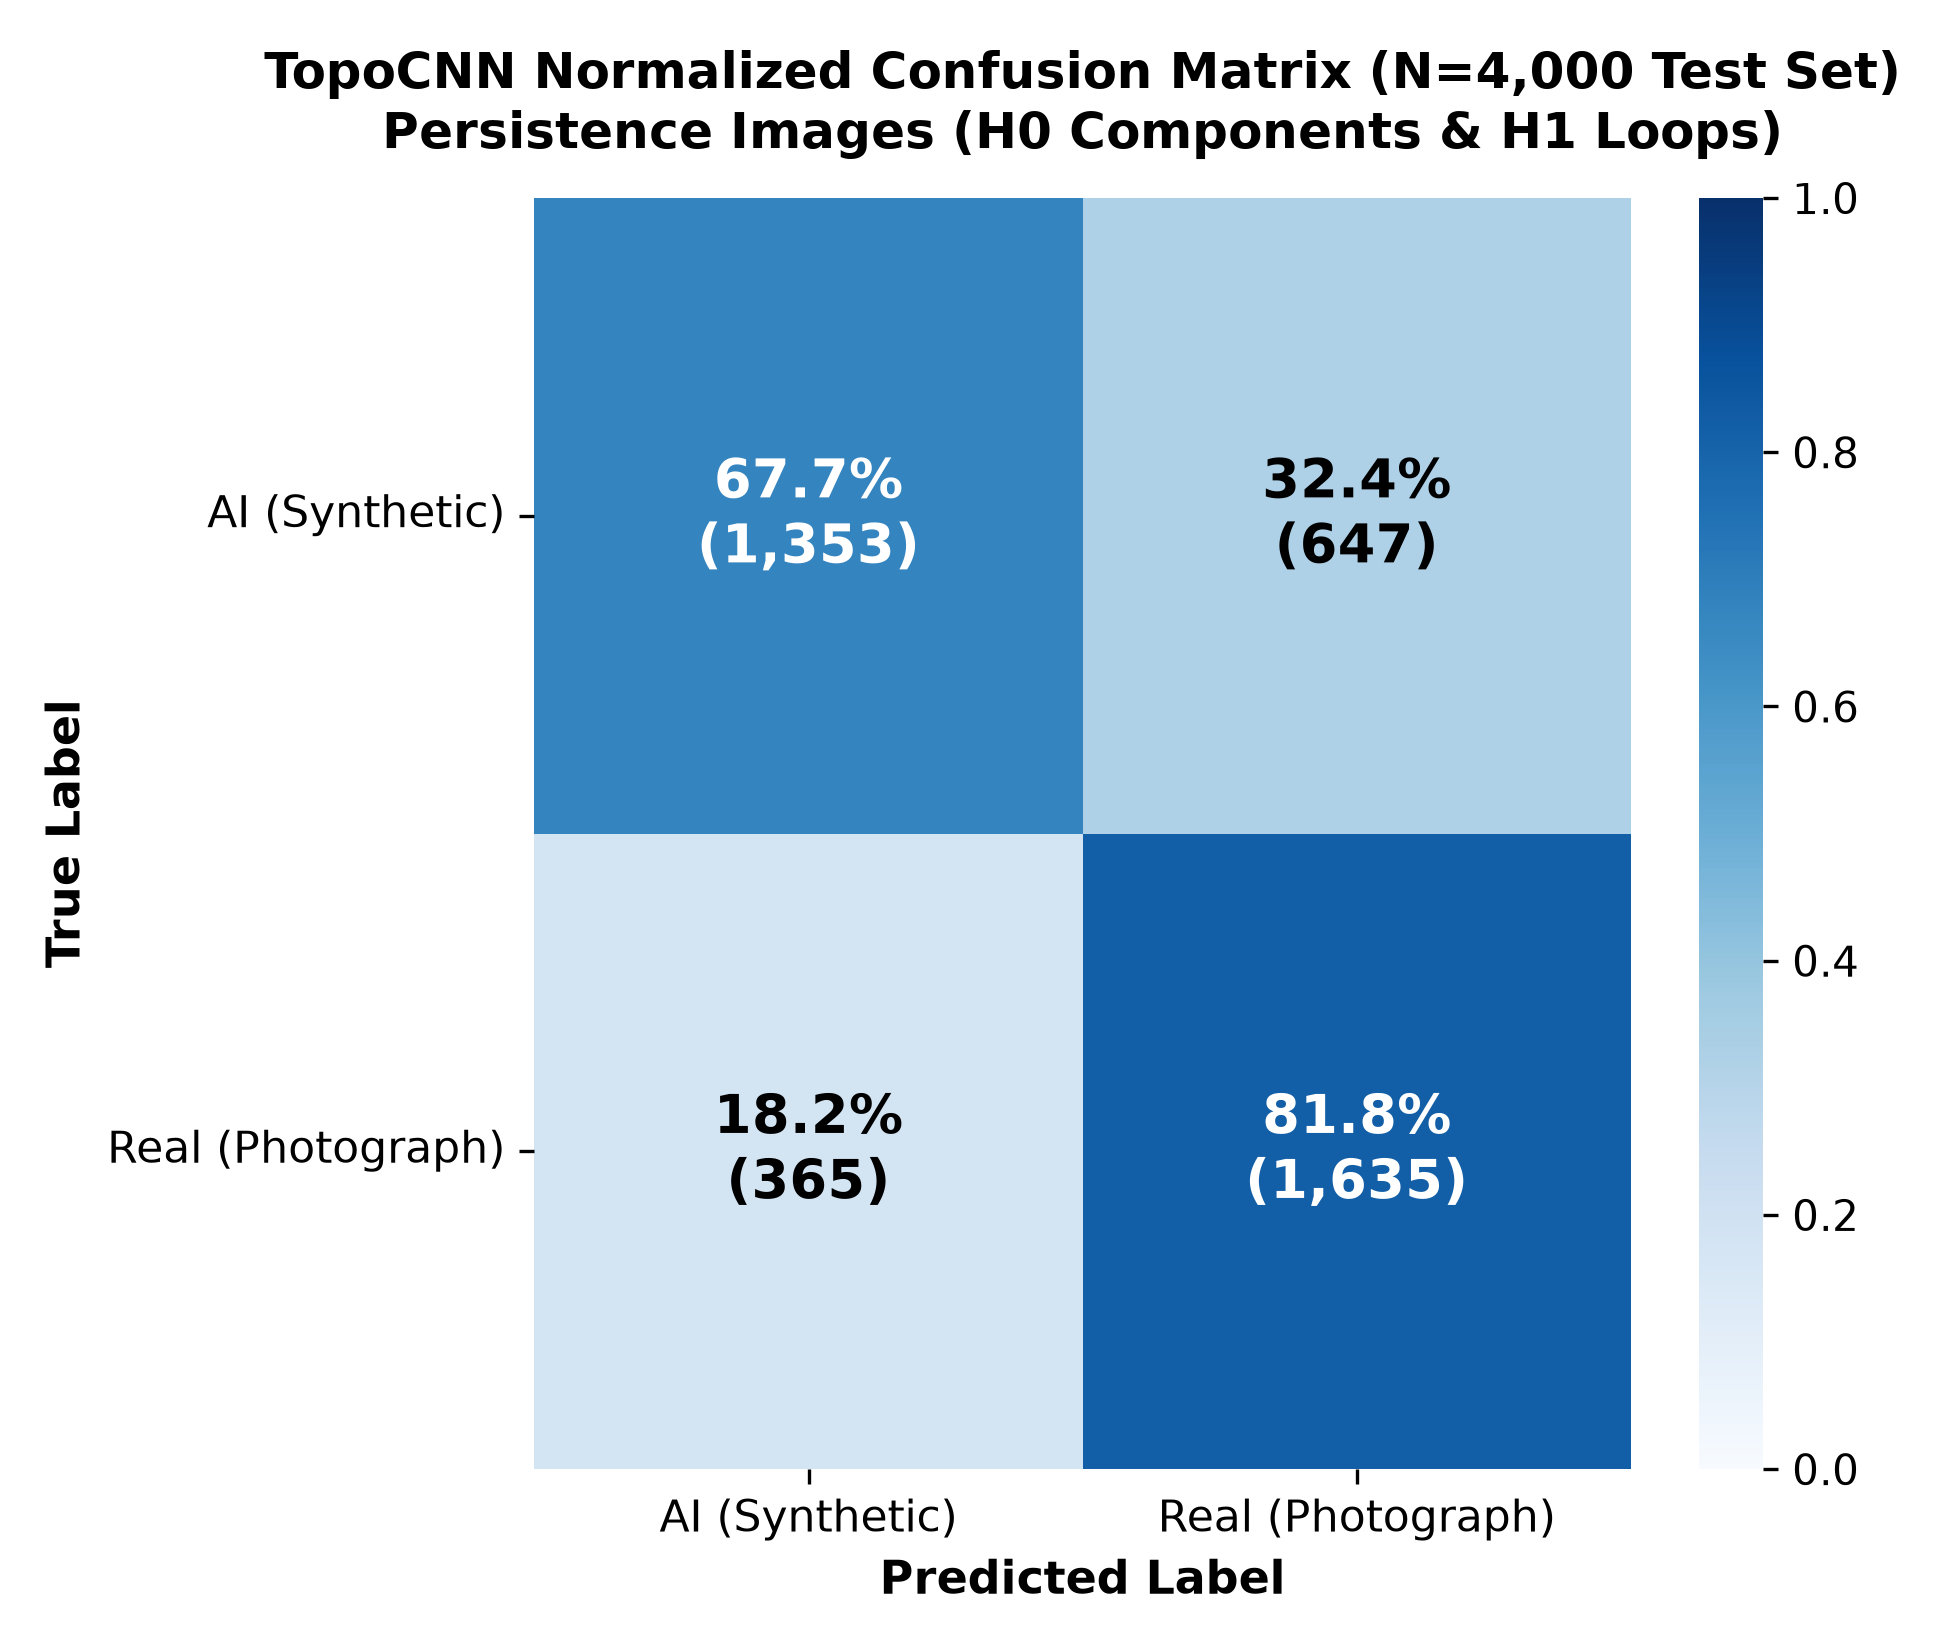
\includegraphics[width=\textwidth]{figures/cnn_confusion_matrix.png}
        \caption{TopoCNN normalized confusion matrix.}
        \label{fig:cnn_cm}
    \end{subfigure}
    \caption{Empirical evaluation of continuous topological learning ($N=4{,}000$): (a) Receiver Operating Characteristic comparison demonstrating the substantial +0.0615 AUC margin of TopoCNN (crimson curve) over all 1D tabular baselines, and (b) TopoCNN confusion matrix demonstrating 81.75\% sensitivity on authentic photography.}
    \label{fig:cnn_eval_combined}
\end{figure}

\subsection{Why 2D Persistence Convolutions Outperform 1D Summaries}
The saved metrics show the following improvements on this internal holdout:
\begin{enumerate}
    \item \textbf{Observed ROC-AUC Gain ($0.7789 \to 0.8404$, $+0.0615$)}: As depicted in Figure~\ref{fig:roc_with_cnn}, TopoCNN has a larger area under its ROC curve; this does not imply dominance at every threshold. While the best tabular model (LightGBM) plateaued at $0.7789$ AUC, TopoCNN surpasses $0.8400$, consistent with useful distributional information in the sampled surfaces. Representation and classifier architecture both change, so the gain cannot be attributed to the representation alone.
    \item \textbf{Increased Accuracy ($70.03\% \to 74.70\%$, $+4.67\%$)}: By learning spatial convolutional filters over birth-lifetime space, TopoCNN detects localized patterns of point accumulation (for example, differences in the density of short- and long-lived features).
    \item \textbf{Elevated Sensitivity ($81.75\%$ Real Photographic Recall)}: As shown in the confusion matrix (Figure~\ref{fig:cnn_cm}), TopoCNN correctly identifies $1{,}635$ out of $2{,}000$ authentic photographs ($81.75\%$ recall, up from $74.85\%$ in LightGBM), leaving 365 real images misclassified. The result does not establish reliability outside this dataset.
    \item \textbf{Lower Brier Score (Brier Score $0.1657$ vs. $0.1911$)}: The Brier score drops by approximately $13.3\%$. It measures overall probabilistic prediction error; a lower score alone does not establish better calibration, which requires separate evaluation.
\end{enumerate}

% ==============================================================================
\section{Interpretation and Limitations}
The observations show distributional differences between the two CIFAKE classes. Possible explanations include differences in textures, image processing, capture pipelines, and image generation. The experiment does not isolate these factors. In particular, it does not measure photon shot noise, attribute individual loops to a decoder operation, or prove that physical and synthetic images have universally distinct topology.

\paragraph{Evaluation scope.} The 20,000-image upstream test partition is re-split into an internal training/validation/holdout experiment. These results must not be presented as a model trained on CIFAKE's official 100,000-image training partition and evaluated on its official 20,000-image test partition. Distribution exploration and SHAP analysis also use holdout observations; confirmation on a new untouched dataset is needed.

\paragraph{Comparisons and robustness.} No raw-pixel CNN baseline, cross-generator evaluation, repeated-seed uncertainty interval, or controlled compression/blur study is included in the saved outputs. The improved CNN metrics compare both a new representation and a new classifier. SHAP explains a fitted XGBoost model, not physical causation. The reported CNN recall treats real photographs as the positive class.

\paragraph{Reproducibility.} The split uses random seed 42, but the original CNN code does not seed PyTorch initialization or data shuffling. Therefore retraining is not expected to reproduce the exact saved metrics. Execution times describe one local run. The accompanying workspace includes the code, environment inventory, saved summary metrics, figures, and a verification of the stored prediction metrics, while raw images and model checkpoints are obtained or generated separately.

% ==============================================================================
\section{Research Roadmap and Future Directions}
% ==============================================================================

With the formulation of continuous 2D Persistence Images and the successful benchmark of TopoCNN, the project roadmap targets the following extensions:

\begin{enumerate}
    \item \textbf{Cross-Generator Generalization}:
    Evaluate whether the 2D topological signatures learned on Stable Diffusion generalize zero-shot to other generative paradigms (e.g., Midjourney, DALL-E 3, Flux, and GAN-based architectures).
    \item \textbf{Multimodal Hybridization (Topology + Frequency)}:
    Integrate 2D Persistence Images with Fourier transform / DCT spectral signatures into a multi-branch forensic network, combining geometric manifold invariants with frequency-domain forensic cues.
    \item \textbf{Adversarial and Perturbation Robustness}:
    Test the stability of TopoCNN under common real-world post-processing perturbations, including JPEG compression, Gaussian blurring, and adversarial noise injection.
\end{enumerate}

% ==============================================================================
\section{Conclusion}
Cubical persistent homology provides informative descriptors for the real and synthetic image classes in the examined CIFAKE sample. Sixteen scalar features support approximately 70\% accuracy, and a compact CNN on sampled two-channel persistence surfaces reaches 74.70\% accuracy and 0.8404 ROC-AUC on the shared internal holdout. These saved results motivate further work on topological representations. The next steps are an untouched evaluation following the official dataset split, suitable pixel-based baselines, repeated runs, and explicit robustness and cross-generator tests.

% ==============================================================================
\begin{thebibliography}{99}
\bibitem{bird2023cifake}
J.~J. Bird and A.~Lotfi, ``CIFAKE: Image classification and explainable identification of AI-generated synthetic images,'' \emph{IEEE Access}, vol.~12, pp.~15602--15613, 2024.

\bibitem{rombach2022high}
R.~Rombach, A.~Blattmann, D.~Lorenz, P.~Esser, and B.~Ommer, ``High-resolution image synthesis with latent diffusion models,'' in \emph{Proceedings of the IEEE/CVF Conference on Computer Vision and Pattern Recognition (CVPR)}, pp.~10684--10695, 2022.

\bibitem{edelsbrunner2000topological}
H.~Edelsbrunner, D.~Letscher, and A.~Zomorodian, ``Topological persistence and simplification,'' \emph{Discrete \& Computational Geometry}, vol.~28, no.~4, pp.~511--533, 2002.

\bibitem{kaczynski2004computational}
T.~Kaczynski, K.~Mischaikow, and M.~Mrozek, \emph{Computational Homology}, Applied Mathematical Sciences, vol.~157, Springer, 2004.

\bibitem{atienza2019stability}
N.~Atienza, R.~Gonzalez-Diaz, and M.~Soriano-Trigueros, ``On the stability of persistent entropy and its applications to image analysis,'' \emph{Pattern Recognition Letters}, vol.~128, pp.~433--440, 2019.

\bibitem{bubenik2015statistical}
P.~Bubenik, ``Statistical topological data analysis using persistence landscapes,'' \emph{Journal of Machine Learning Research}, vol.~16, no.~1, pp.~77--102, 2015.

\bibitem{adams2017persistence}
H.~Adams, T.~Emerson, M.~Kirby, R.~Neville, C.~Peterson, P.~Shipman, S.~Chepushtanova, E.~Hanson, F.~Motta, and L.~Ziegelmeier, ``Persistence images: A stable vector representation of persistent homology,'' \emph{Journal of Machine Learning Research}, vol.~18, no.~8, pp.~1--35, 2017.

\bibitem{gudhi2024}
The GUDHI Project, ``GUDHI User and Reference Manual,'' Inria, 2024. [Online]. Available: \url{https://gudhi.inria.fr/}

\bibitem{lundberg2017unified}
S.~M. Lundberg and S.-I. Lee, ``A unified approach to interpreting model predictions,'' in \emph{Advances in Neural Information Processing Systems (NeurIPS)}, vol.~30, pp.~4765--4774, 2017.

\bibitem{chen2016xgboost}
T.~Chen and C.~Guestrin, ``XGBoost: A scalable tree boosting system,'' in \emph{Proceedings of the ACM SIGKDD International Conference on Knowledge Discovery and Data Mining}, pp.~785--794, 2016.

\bibitem{ke2017lightgbm}
G.~Ke, Q.~Meng, T.~Finley, T.~Wang, W.~Chen, W.~Ma, Q.~Ye, and T.-Y. Liu, ``LightGBM: A highly efficient gradient boosting decision tree,'' in \emph{Advances in Neural Information Processing Systems (NeurIPS)}, vol.~30, pp.~3146--3154, 2017.

\bibitem{breiman2001random}
L.~Breiman, ``Random forests,'' \emph{Machine Learning}, vol.~45, no.~1, pp.~5--32, 2001.

\bibitem{cortes1995support}
C.~Cortes and V.~Vapnik, ``Support-vector networks,'' \emph{Machine Learning}, vol.~20, no.~3, pp.~273--297, 1995.

\bibitem{hendrycks2016gaussian}
D.~Hendrycks and K.~Gimpel, ``Gaussian error linear units (GELUs),'' \emph{arXiv preprint arXiv:1606.08415}, 2016.
\end{thebibliography}

\end{document}
